\documentclass[11pt]{article}

% ── Encoding & lingua ────────────────────────────────────────
\usepackage[T1]{fontenc}
\usepackage[utf8]{inputenc}
\usepackage[italian]{babel}

% ── Layout pagina ────────────────────────────────────────────
\usepackage[
  a4paper,
  top=2.4cm, bottom=2.4cm,
  left=2.5cm, right=2.5cm
]{geometry}

% ── Matematica ───────────────────────────────────────────────
\usepackage{amsmath, amssymb}

% ── Grafica ──────────────────────────────────────────────────
\usepackage{graphicx}
\graphicspath{{../parte_A/}{../parte_B/}{../parte_C/}{./}}

% ── Tabelle ──────────────────────────────────────────────────
\usepackage{booktabs}
\usepackage{array}
\usepackage{multirow}

% ── Colori ───────────────────────────────────────────────────
\usepackage[dvipsnames]{xcolor}
\definecolor{uniblue}{RGB}{0,84,159}

% ── Hyperlink ────────────────────────────────────────────────
\usepackage[
  colorlinks=true,
  linkcolor=uniblue,
  urlcolor=uniblue,
  citecolor=uniblue
]{hyperref}

% ── Spaziatura & paragrafi ───────────────────────────────────
\usepackage{setspace}
\setstretch{1.15}
\setlength{\parindent}{0pt}
\setlength{\parskip}{0.55em}

% ── Didascalie ───────────────────────────────────────────────
\usepackage[font=small, labelfont=bf, justification=centering]{caption}

% ── Sezioni ──────────────────────────────────────────────────
\usepackage{titlesec}
\titleformat{\section}{\large\bfseries\color{uniblue}}{\thesection.}{0.6em}{}[\vspace{-0.3em}\rule{\linewidth}{0.6pt}]
\titleformat{\subsection}{\normalsize\bfseries}{\thesubsection}{0.5em}{}
\titlespacing{\section}{0pt}{1.6em}{0.4em}
\titlespacing{\subsection}{0pt}{1em}{0.2em}

% ── Titolo ───────────────────────────────────────────────────
\usepackage{titling}
\pretitle{%
  \begin{center}
  
\includegraphics[height=2.2cm]{logoUnipi_black.png}\\[1.2em]
  \rule{\textwidth}{0.6pt}\\[0.8em]
  \LARGE\bfseries}
\posttitle{%
  \\[0.4em]\rule{\textwidth}{0.6pt}
  \end{center}\vspace{0.5em}}
\preauthor{\begin{center}\large}
\postauthor{\end{center}}
\predate{}
\postdate{}
\date{}

\title{Caso Pratico  EMFI 1}
\author{Leonardo Pratelli\thanks{\texttt{l.pratelli3@studenti.unipi.it}}%
        \quad Sara Albotica\thanks{\texttt{s.albotica@studenti.unipi.it}}}

% ─────────────────────────────────────────────────────────────
\begin{document}
\maketitle
\tableofcontents
\newpage

% ============================================================
\section*{Introduzione}
\addcontentsline{toc}{section}{Introduzione}
% ============================================================

Il presente report risponde alla traccia del Caso Pratico EMFI 1.
Sono stati scaricati da Yahoo Finance i prezzi mensili \emph{adjusted}
(total return, dividendi inclusi) di 10 titoli azionari e indici per
il periodo \textbf{gennaio 2015 -- dicembre 2024} (120 prezzi mensili,
119 rendimenti logaritmici mensili dopo il primo differenziale).

\textbf{Struttura 3-3-3-1.} I titoli sono stati scelti per massimizzare
la diversificazione settoriale:

\begin{center}
\begin{tabular}{llll}
\toprule
\textbf{Settore} & \textbf{Ticker} & \textbf{Azienda} & \textbf{Motivazione} \\
\midrule
Tecnologia   & AAPL & Apple     & Alta capitalizzazione, elevata crescita \\
             & MSFT & Microsoft & Cloud + AI, stabile e crescente \\
             & NVDA & Nvidia    & Semiconduttori/AI, alta volatilità e rendimento \\
Healthcare   & JNJ  & Johnson \& Johnson & Difensivo, dividendi stabili \\
             & PFE  & Pfizer    & Farmaceutico ciclico \\
             & MRK  & Merck     & Oncologia, bassa correlazione con Tech \\
Energy       & XOM  & ExxonMobil & Major petrolifera USA \\
             & CVX  & Chevron   & Diversificata, ottimo dividendo \\
             & BP   & BP plc    & Europea, esposizione diversificata \\
Indice       & \^{}GSPC & S\&P 500 & Proxy portafoglio di mercato (CAPM) \\
\bottomrule
\end{tabular}
\end{center}

\textbf{Tasso risk-free.} Si assume $r_f = 2{,}00\%$ annuo ($0{,}1667\%$
mensile), coerente con la media storica del BOT trimestrale italiano
nel periodo 2015--2024.

\textbf{Nota sui rendimenti.} Il codice calcola rendimenti logaritmici
$r_t = \ln(P_t/P_{t-1})$, che godono di additività temporale.
La teoria di Markowitz è formalmente fondata su rendimenti semplici
($r_p = \mathbf{w}'r$); per dati mensili l'approssimazione
$\ln(1+R)\approx R$ (errore medio $<0{,}5\%$) rende i due approcci
sostanzialmente equivalenti.

% ============================================================
\section{Parte A -- Frontiera Efficiente}
% ============================================================

\subsection{Punto 1 -- Dataset, statistiche descrittive e matrici}

La Tabella~\ref{tab:stats} riassume le statistiche annualizzate
dei 10 titoli/indici calcolate sui 119 rendimenti logaritmici mensili.

\begin{table}[h!]
\centering
\caption{Statistiche annualizzate dei 10 asset (rendimenti log mensili,
periodo 2015-01 -- 2024-12).
SR $= \mu_a / \sigma_a$ con $r_f = 0$ per comparabilità.}
\label{tab:stats}
\begin{tabular}{lrrr}
\toprule
\textbf{Ticker} & \textbf{$\mu$ annuo (\%)} & \textbf{$\sigma$ annua (\%)} & \textbf{Sharpe} \\
\midrule
NVDA  & 57{,}22 & 45{,}50 & 1{,}258 \\
MSFT  & 25{,}18 & 20{,}90 & 1{,}205 \\
AAPL  & 22{,}81 & 27{,}32 & 0{,}835 \\
SP500 & 10{,}90 & 15{,}37 & 0{,}709 \\
MRK   &  8{,}60 & 19{,}42 & 0{,}443 \\
JNJ   &  6{,}49 & 15{,}70 & 0{,}413 \\
CVX   &  7{,}79 & 26{,}77 & 0{,}291 \\
XOM   &  6{,}49 & 27{,}00 & 0{,}240 \\
BP    &  3{,}19 & 25{,}45 & 0{,}125 \\
PFE   &  2{,}85 & 22{,}64 & 0{,}126 \\
\bottomrule
\end{tabular}
\end{table}

NVDA e MSFT dominano per rendimento atteso; MRK e JNJ offrono
la minore volatilità nel settore Healthcare.
Le Figure~\ref{fig:covheat}--\ref{fig:scatter} mostrano la matrice
di varianza-covarianza, la matrice di correlazione e lo scatter
rischio/rendimento.

\begin{figure}[h!]
\centering
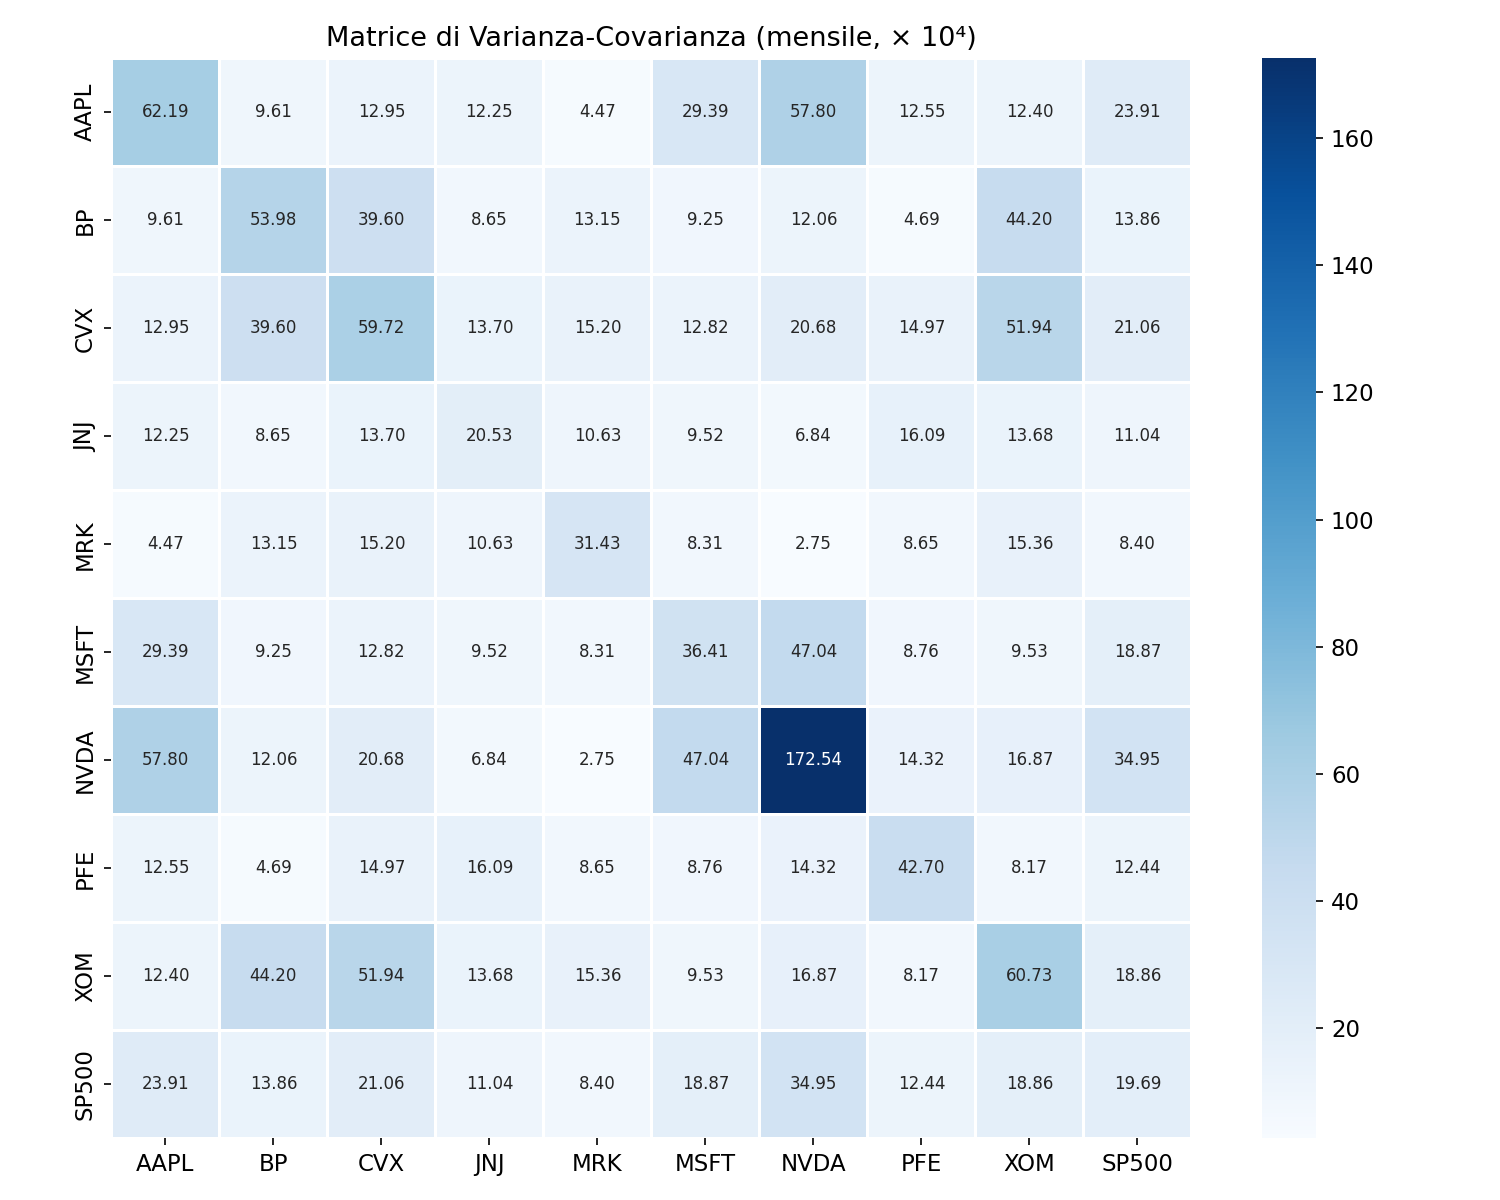
\includegraphics[width=0.82\linewidth]{covariance_heatmap.png}
\caption{Matrice di varianza-covarianza mensile (valori $\times 10^{-4}$).
NVDA presenta la varianza più elevata; le covarianze Tech-Energy
sono più basse di quelle intra-Tech.}
\label{fig:covheat}
\end{figure}

\begin{figure}[h!]
\centering
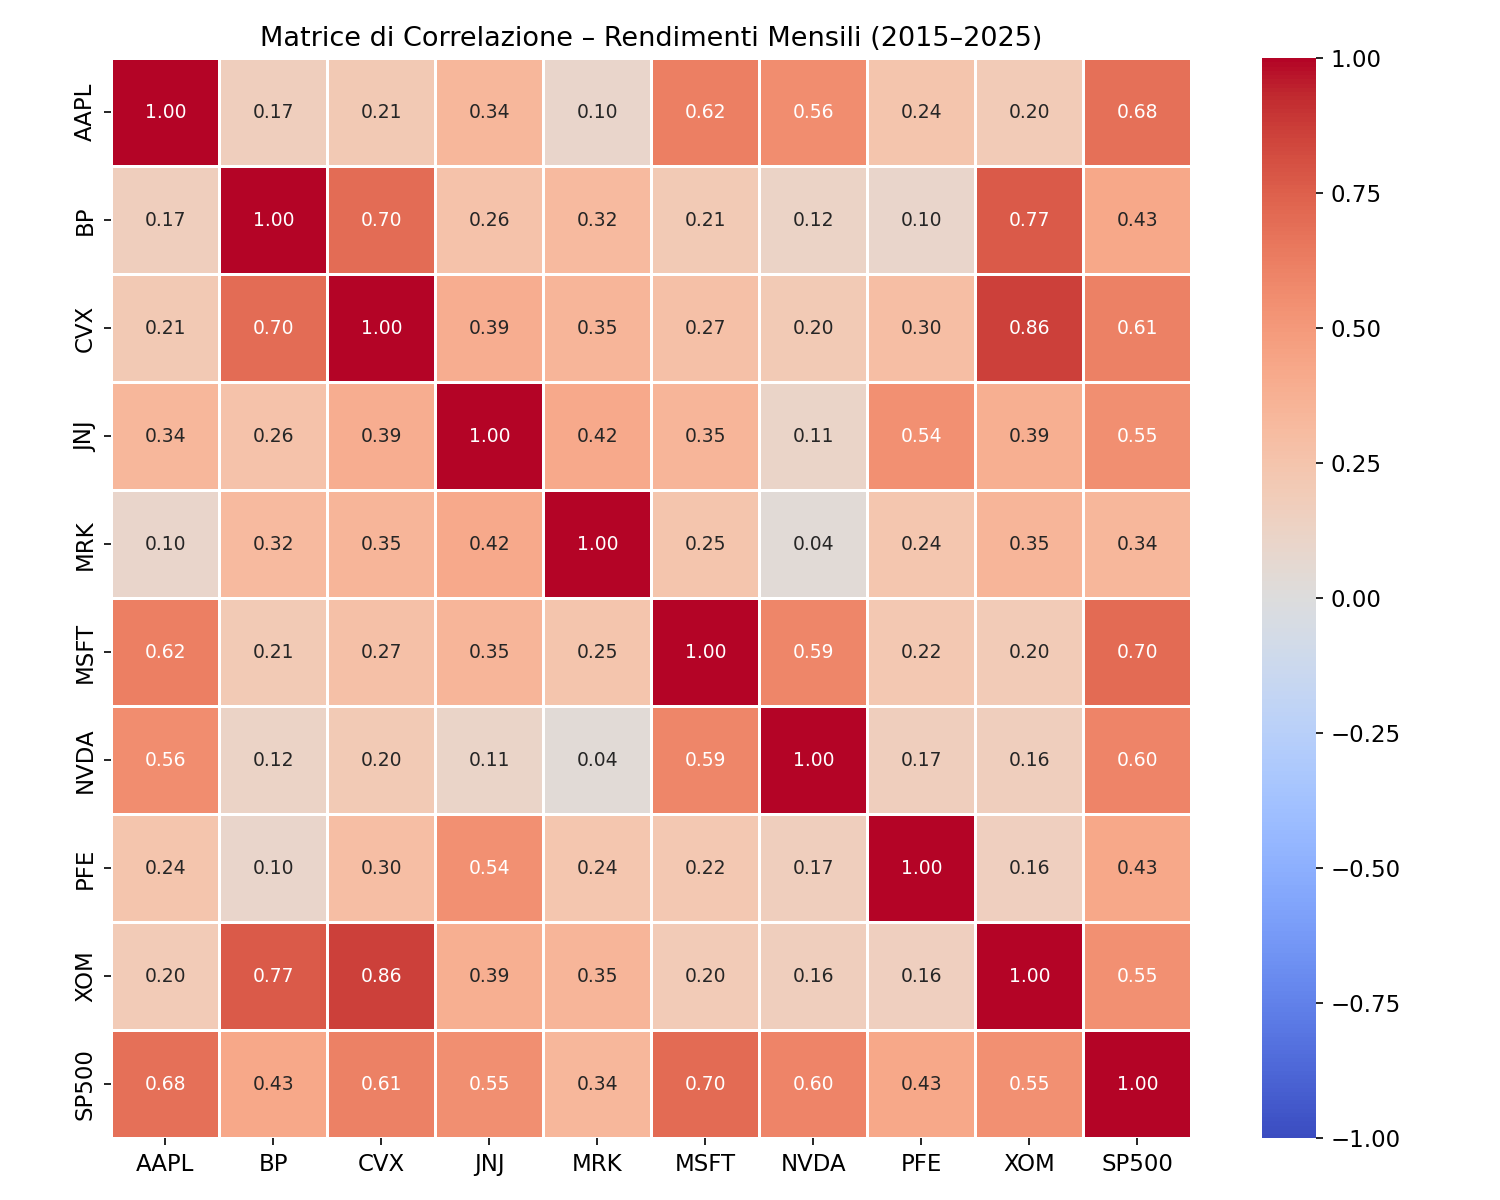
\includegraphics[width=0.82\linewidth]{correlation_heatmap.png}
\caption{Matrice di correlazione. Si notano le alte correlazioni
intra-settore (Tech: NVDA--MSFT $\rho{=}0{,}59$) e le basse
correlazioni inter-settore (NVDA--MRK $\rho{=}0{,}04$), utili
per la diversificazione.}
\label{fig:corheat}
\end{figure}

\begin{figure}[h!]
\centering
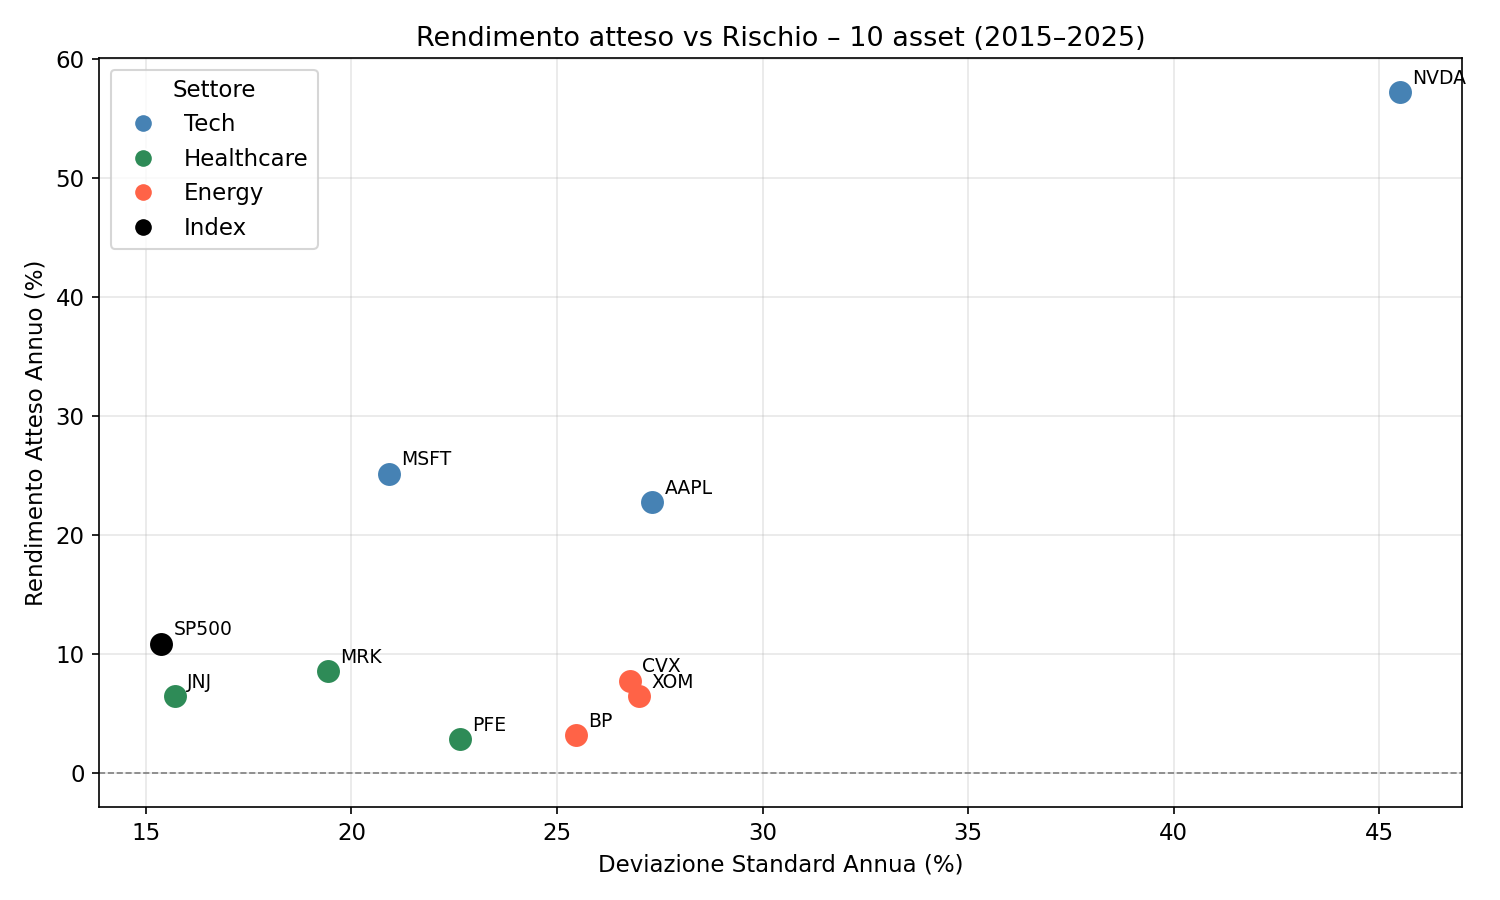
\includegraphics[width=0.78\linewidth]{risk_return_scatter.png}
\caption{Scatter rendimento atteso annuo vs deviazione standard annua
per i 10 asset. NVDA e MSFT si trovano nella zona in alto a destra
(alto rischio, alto rendimento); JNJ e SP500 nella zona in basso
a sinistra (difensivi).}
\label{fig:scatter}
\end{figure}

\subsection{Punto 2 -- Frontiera efficiente: approccio analitico e numerico}

\textbf{Selezione dei 5 titoli.}
Per la costruzione della frontiera sono stati scelti
\textbf{NVDA, MSFT, JNJ, MRK, XOM}, in base a tre criteri:
(i) massima diversificazione settoriale (Tech + Healthcare + Energy);
(ii) basse correlazioni inter-settore
($\rho_{\text{NVDA,MRK}}{=}0{,}037$,
 $\rho_{\text{NVDA,XOM}}{=}0{,}165$);
(iii) spread nel profilo rischio/rendimento (da NVDA con SR${\approx}$1,26
a XOM con SR${\approx}$0,24).

\textbf{Approccio analitico.}
Con $N{=}5$ asset, la frontiera media-varianza senza vincoli si ottiene
dai quattro scalari di Markowitz:
\[
  A = \mathbf{1}'\Sigma^{-1}\boldsymbol{\mu}, \quad
  B = \boldsymbol{\mu}'\Sigma^{-1}\boldsymbol{\mu}, \quad
  C = \mathbf{1}'\Sigma^{-1}\mathbf{1}, \quad
  D = BC - A^2
\]
i cui valori stimati sono riportati nella Tabella~\ref{tab:markowitz}.
La frontiera è la curva $\sigma_p^2(\mu_p) = (C\mu_p^2 - 2A\mu_p + B)/D$.

\begin{table}[h!]
\centering
\caption{Scalari di Markowitz (valori mensili).}
\label{tab:markowitz}
\begin{tabular}{cccc}
\toprule
$A$ & $B$ & $C$ & $D$ \\
\midrule
6{,}0954 & 0{,}1654 & 652{,}37 & 70{,}76 \\
\bottomrule
\end{tabular}
\end{table}

Il \textbf{Portafoglio di Minima Varianza Globale (GMV)} ha pesi
$\mathbf{w}^{\text{GMV}} = \Sigma^{-1}\mathbf{1}/C$,
rendimento $\mu_{\text{GMV}} = A/C$ e varianza $\sigma^2_{\text{GMV}} = 1/C$,
come derivato nelle slide (EMFI\_2, eq.~10--11).
Le caratteristiche numeriche sono riportate nella Tabella~\ref{tab:gmv}.

\begin{table}[h!]
\centering
\caption{Portafoglio di Minima Varianza Globale (GMV), valori annualizzati.}
\label{tab:gmv}
\begin{tabular}{lrrrrrrr}
\toprule
 & \multicolumn{5}{c}{\textbf{Pesi}} & \textbf{$\mu$ (\%)} & \textbf{$\sigma$ (\%)} \\
\cmidrule(lr){2-6}
 & NVDA & MSFT & JNJ & MRK & XOM & & \\
\midrule
GMV & $-0{,}001$ & $+0{,}228$ & $+0{,}486$ & $+0{,}240$ & $+0{,}047$ & 11{,}21 & 13{,}56 \\
\bottomrule
\end{tabular}
\end{table}

\textbf{Verifica numerica.} La frontiera è stata calcolata
indipendentemente via ottimizzazione SLSQP su 50 punti equidistanti
in $\mu_p$: tutti i punti numerici coincidono con la curva analitica,
confermando la correttezza dei calcoli. La Figura~\ref{fig:frontier2}
mostra le due frontiere sovrapposte.

\begin{figure}[h!]
\centering
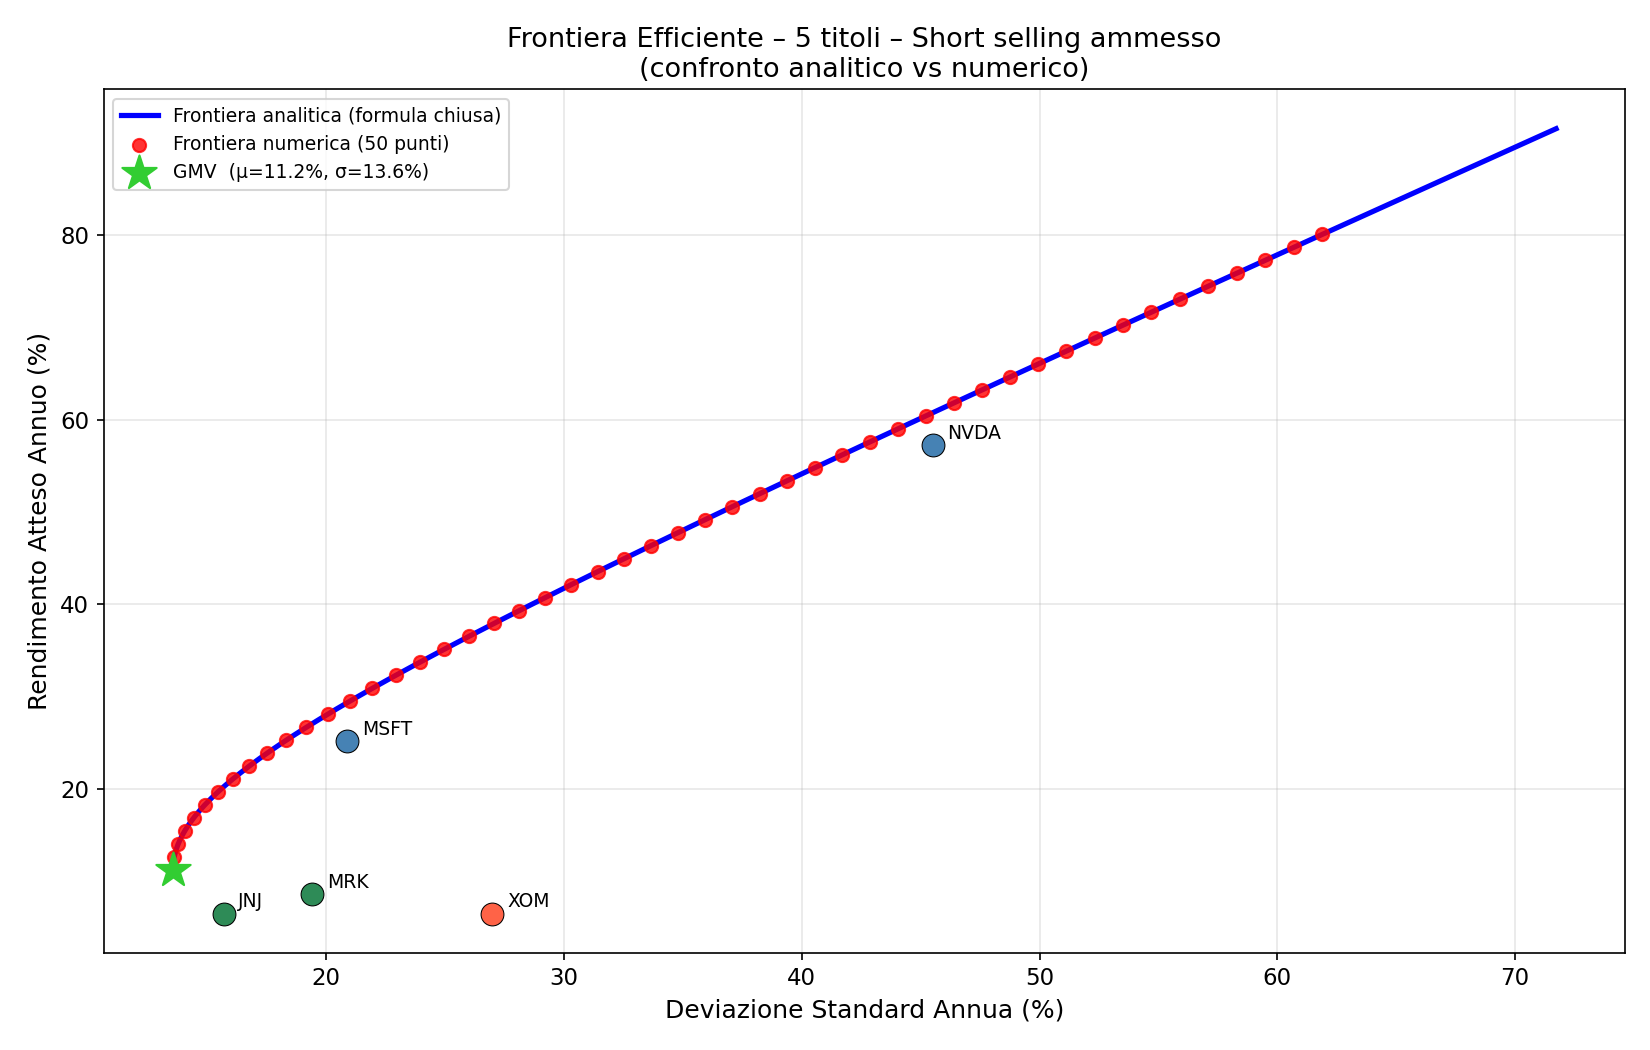
\includegraphics[width=0.82\linewidth]{efficient_frontier_A2.png}
\caption{Frontiera efficiente analitica (curva continua) e punti
numerici SLSQP (cerchi). La perfetta sovrapposizione conferma
la coerenza tra le due metodologie.}
\label{fig:frontier2}
\end{figure}

\subsection{Punto 3 -- Frontiera long-only (no short selling)}

Imponendo il vincolo $w_i \geq 0$ per ogni $i$, la frontiera
long-only è calcolata numericamente (SLSQP). La
Figura~\ref{fig:frontier3} mostra il confronto con quella
senza vincoli.

\begin{figure}[h!]
\centering
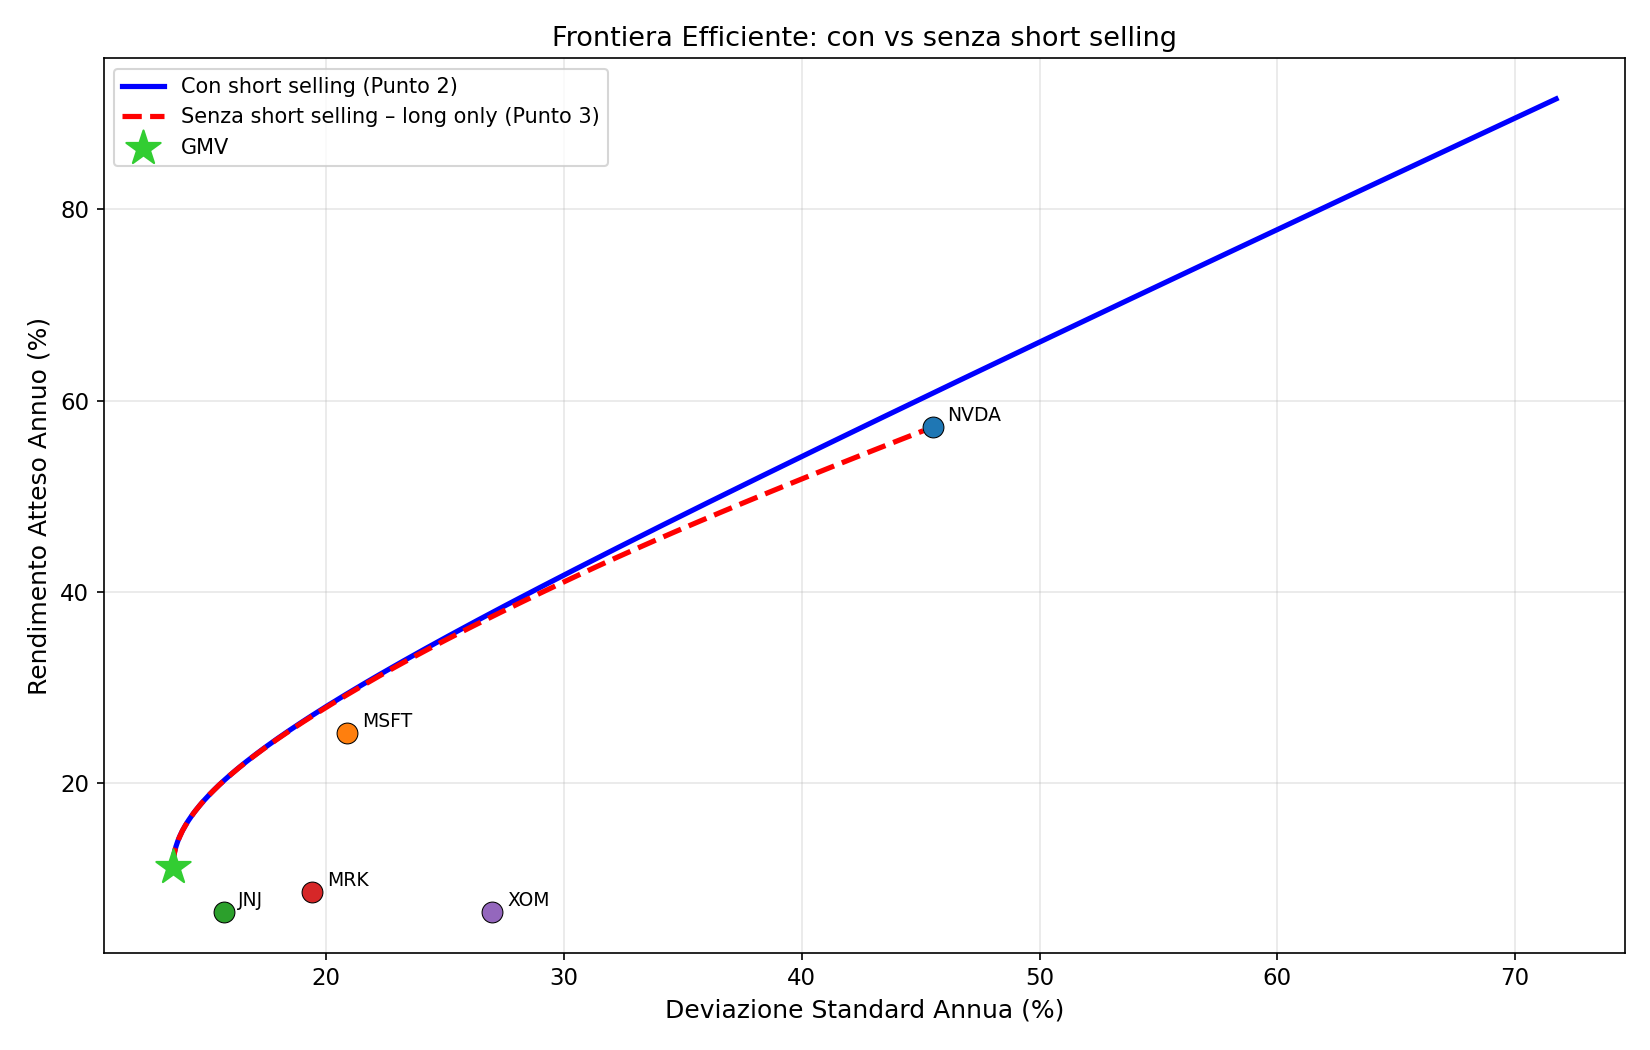
\includegraphics[width=0.82\linewidth]{efficient_frontier_A3_comparison.png}
\caption{Confronto frontiera con short selling (blu) e long-only
(arancio). Il vincolo $w_i \geq 0$ riduce l'insieme delle
opportunità: a parità di rischio, il rendimento massimo
raggiungibile è inferiore, e la frontiera long-only è
interamente contenuta a destra di quella senza vincoli.}
\label{fig:frontier3}
\end{figure}

L'impossibilità di vendere allo scoperto limita la copertura delle
correlazioni positive intra-settore (es.\ MSFT--NVDA $\rho{=}0{,}59$),
riducendo i benefici della diversificazione.

\subsection{Punto 4 -- Portafoglio di mercato e frontiera efficiente}

L'\textbf{S\&P~500} è usato come proxy del portafoglio di mercato:
$\mu_m^{\text{ann}} = 10{,}90\%$, $\sigma_m^{\text{ann}} = 15{,}37\%$.
A parità di deviazione standard ($\sigma = 15{,}37\%$), il portafoglio
sulla frontiera degli stessi 5 titoli offre $\mu_{\text{front}} = 19{,}47\%$,
con un \textbf{differenziale di rendimento di $+8{,}56\%$ annuo}.
L'S\&P~500 \emph{non si trova} sulla frontiera efficiente dei 5 titoli
scelti: ciò è atteso, poiché la frontiera è costruita su un
sottoinsieme dei 10 titoli disponibili e ottimizzata sul campione storico.

\begin{figure}[h!]
\centering
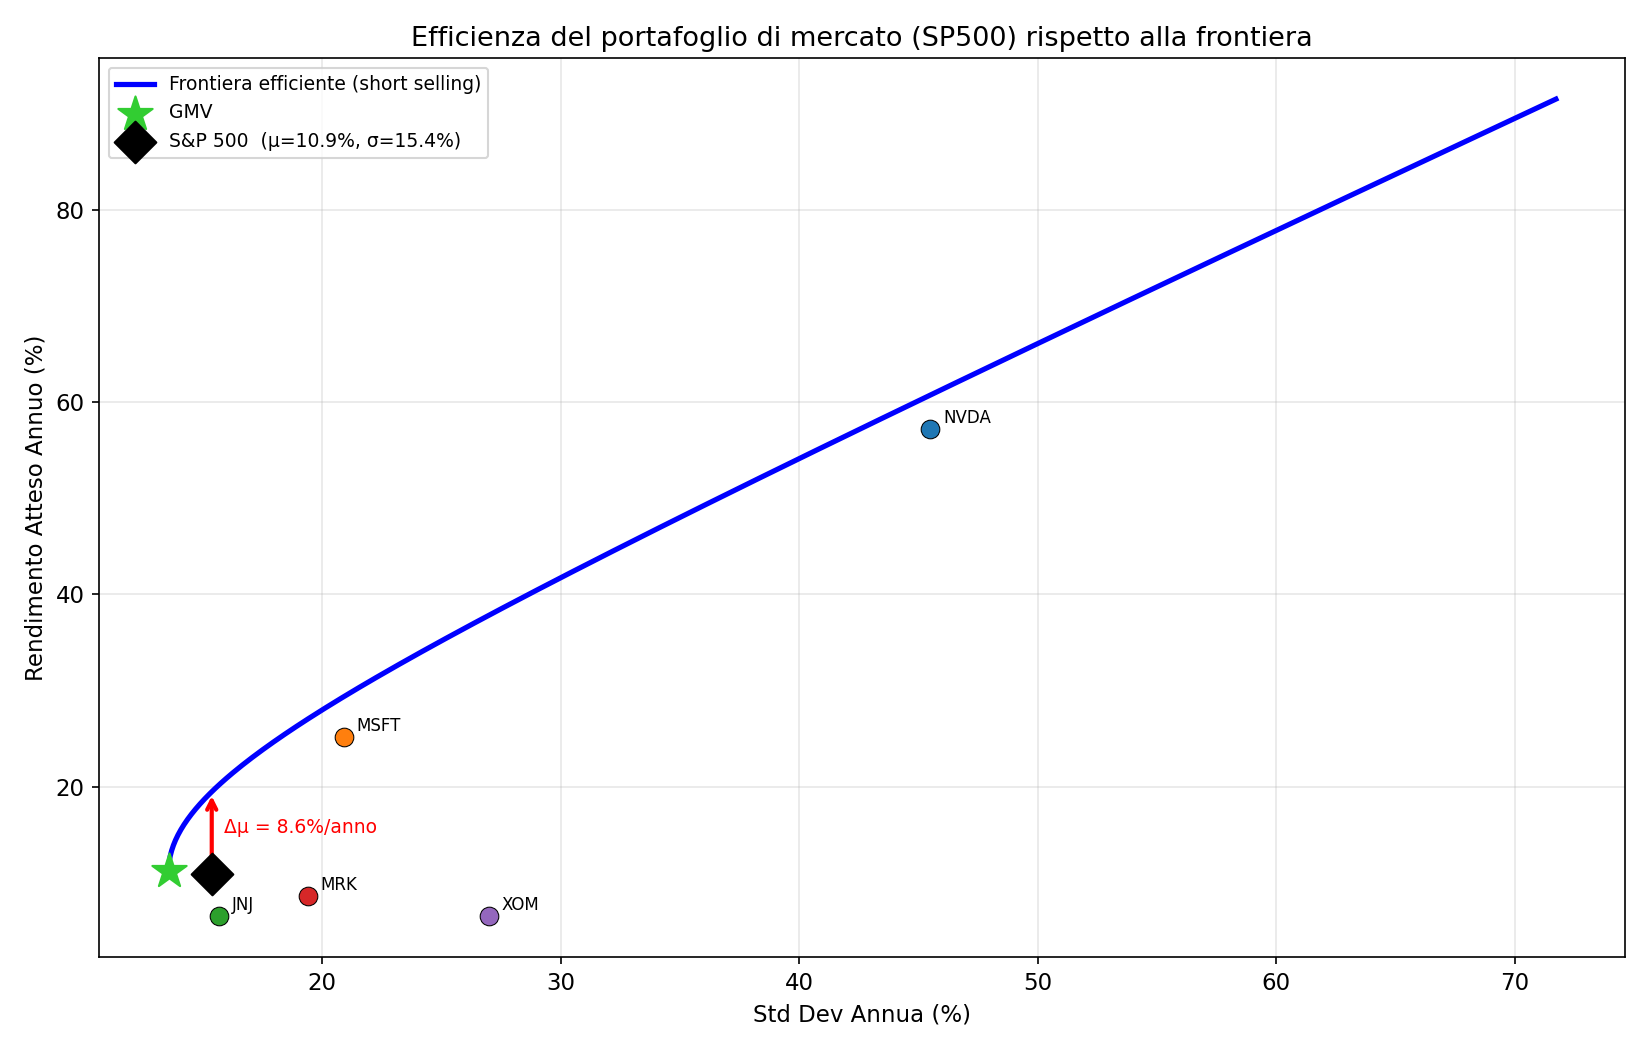
\includegraphics[width=0.82\linewidth]{market_portfolio_A4.png}
\caption{S\&P~500 rispetto alla frontiera efficiente: la freccia
verticale evidenzia il rendimento aggiuntivo disponibile a parità
di rischio ($\Delta\mu = +8{,}56\%$ annuo).}
\label{fig:market4}
\end{figure}

\subsection{Punto 5 -- Confronto con portafogli benchmark}

La Tabella~\ref{tab:benchmarks} confronta le statistiche dei
portafogli benchmark con la frontiera efficiente.

\begin{table}[h!]
\centering
\caption{Confronto portafogli benchmark vs frontiera efficiente (valori annualizzati).
\textit{Rendimento perso} = differenza rispetto al portafoglio sulla frontiera
con la stessa $\sigma$.}
\label{tab:benchmarks}
\begin{tabular}{lrrrr}
\toprule
\textbf{Portafoglio} & \textbf{$\mu$ (\%)} & \textbf{$\sigma$ (\%)} & \textbf{$\mu_{\text{front}}$ (\%)} & \textbf{Rend.\ perso (\%)} \\
\midrule
GMV       & 11{,}21 & 13{,}56 & --     & -- \\
EW5       & 20{,}80 & 17{,}01 & 22{,}92 & 2{,}12 \\
EW10      & 15{,}15 & 15{,}89 & 20{,}66 & 5{,}51 \\
S\&P~500  & 10{,}90 & 15{,}37 & 19{,}47 & 8{,}56 \\
\bottomrule
\end{tabular}
\end{table}

Il portafoglio \textbf{EW5} è il più vicino alla frontiera (perde solo
il 2{,}12\%), grazie alla forte concentrazione nei 5 titoli selezionati
che includono NVDA e MSFT con i Sharpe più elevati.
\textbf{EW10} e \textbf{S\&P~500}, diluendo il peso di NVDA e MSFT con
asset meno performanti (PFE, BP), perdono rispettivamente il 5{,}51\%
e l'8{,}56\% di rendimento annuo rispetto alla frontiera efficiente.

\begin{figure}[h!]
\centering
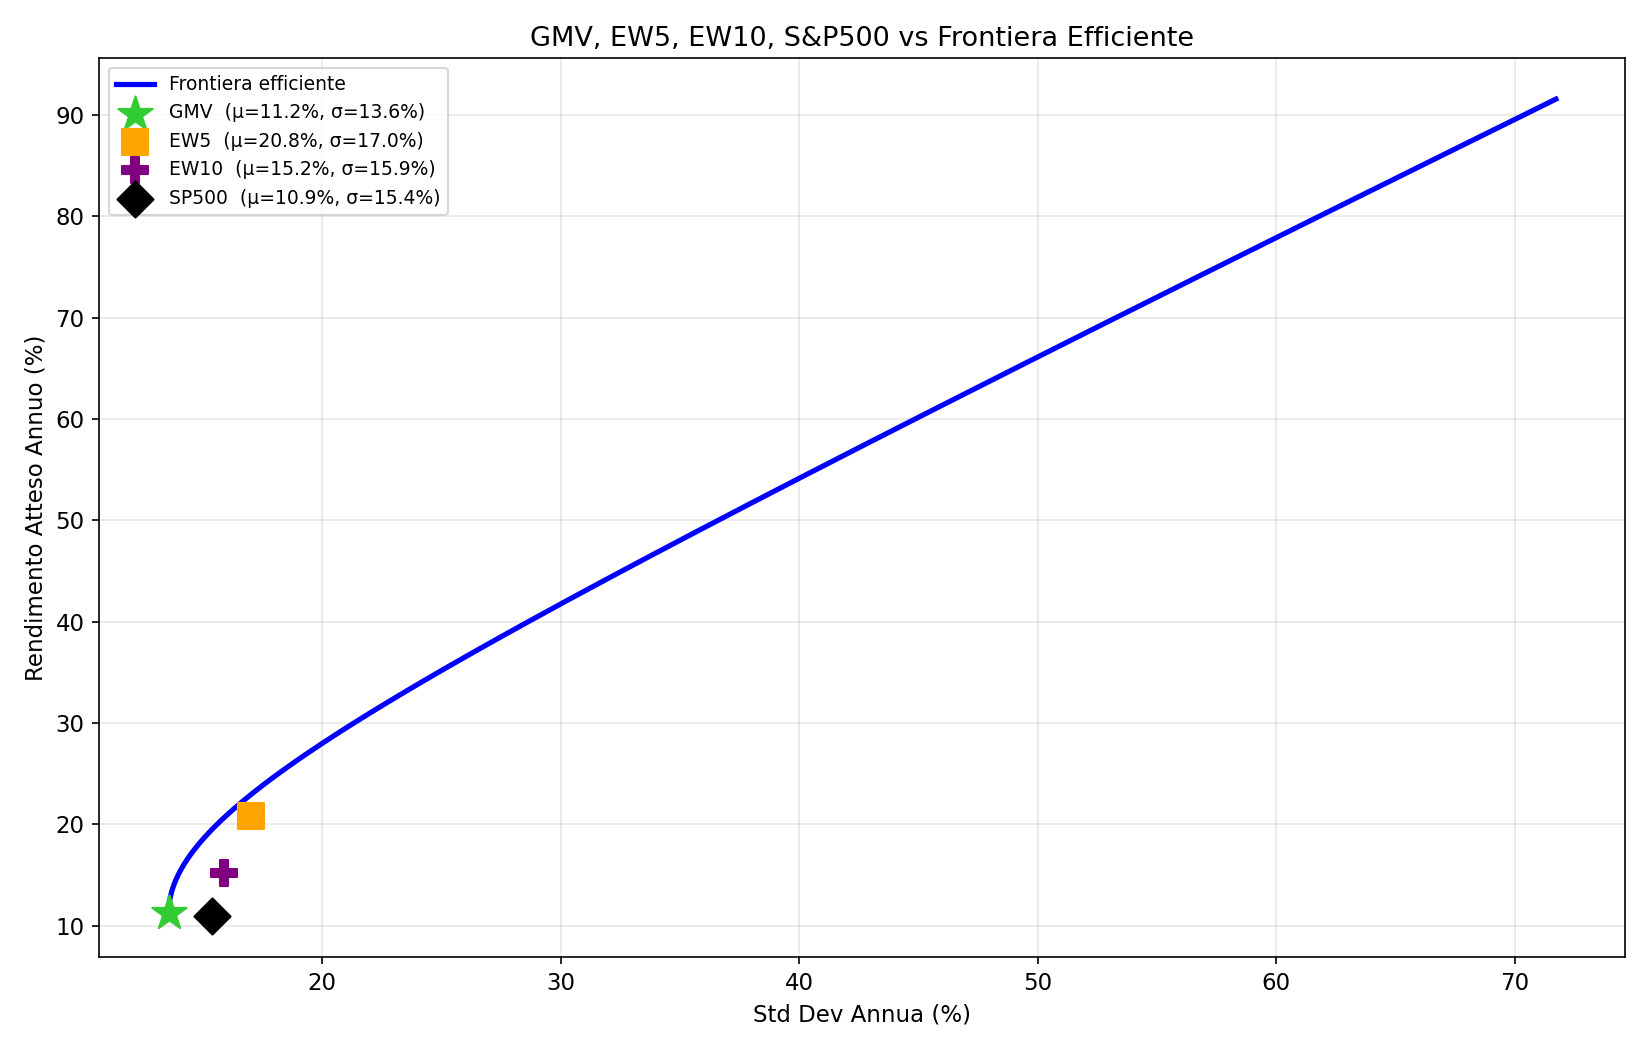
\includegraphics[width=0.82\linewidth]{benchmarks_A5.png}
\caption{Posizionamento dei portafogli benchmark rispetto alla
frontiera efficiente. La distanza verticale di ciascun punto
dalla curva rappresenta il \emph{rendimento perso}.}
\label{fig:bench5}
\end{figure}

\subsection{Punto 6 -- Capital Market Line e portafoglio di tangenza}

Introducendo l'asset privo di rischio ($r_f = 2{,}00\%$ annuo), la
frontiera si estende alla \textbf{Capital Market Line (CML)}.
Il \textbf{portafoglio di tangenza} massimizza lo Sharpe Ratio ed
è dato dalla formula analitica:
\[
  \mathbf{w}_{\text{tan}} =
  \frac{\Sigma^{-1}(\boldsymbol{\mu} - r_f\mathbf{1})}
       {\mathbf{1}'\,\Sigma^{-1}(\boldsymbol{\mu} - r_f\mathbf{1})}
\]

Le caratteristiche del portafoglio di tangenza sono riportate
nella Tabella~\ref{tab:tangenza}.

\begin{table}[h!]
\centering
\caption{Portafoglio di tangenza ($r_f = 2{,}00\%$ annuo), valori annualizzati.}
\label{tab:tangenza}
\begin{tabular}{lrrrrrrrrr}
\toprule
 & \multicolumn{5}{c}{\textbf{Pesi}} & \textbf{$\mu_{\text{tan}}$ (\%)} & \textbf{$\sigma_{\text{tan}}$ (\%)} & \textbf{SR} \\
\cmidrule(lr){2-6}
 & NVDA & MSFT & JNJ & MRK & XOM & & & \\
\midrule
Tangenza & $+0{,}396$ & $+0{,}540$ & $-0{,}070$ & $+0{,}254$ & $-0{,}120$ & 37{,}20 & 26{,}51 & 1{,}328 \\
\bottomrule
\end{tabular}
\end{table}

NVDA e MSFT ricevono i pesi maggiori, coerentemente con i loro
Sharpe individuali elevati. JNJ e XOM hanno peso leggermente
negativo (short selling), segno che il loro apporto marginale
al portafoglio è negativo dopo aver ottimizzato lo Sharpe Ratio.

\begin{figure}[h!]
\centering
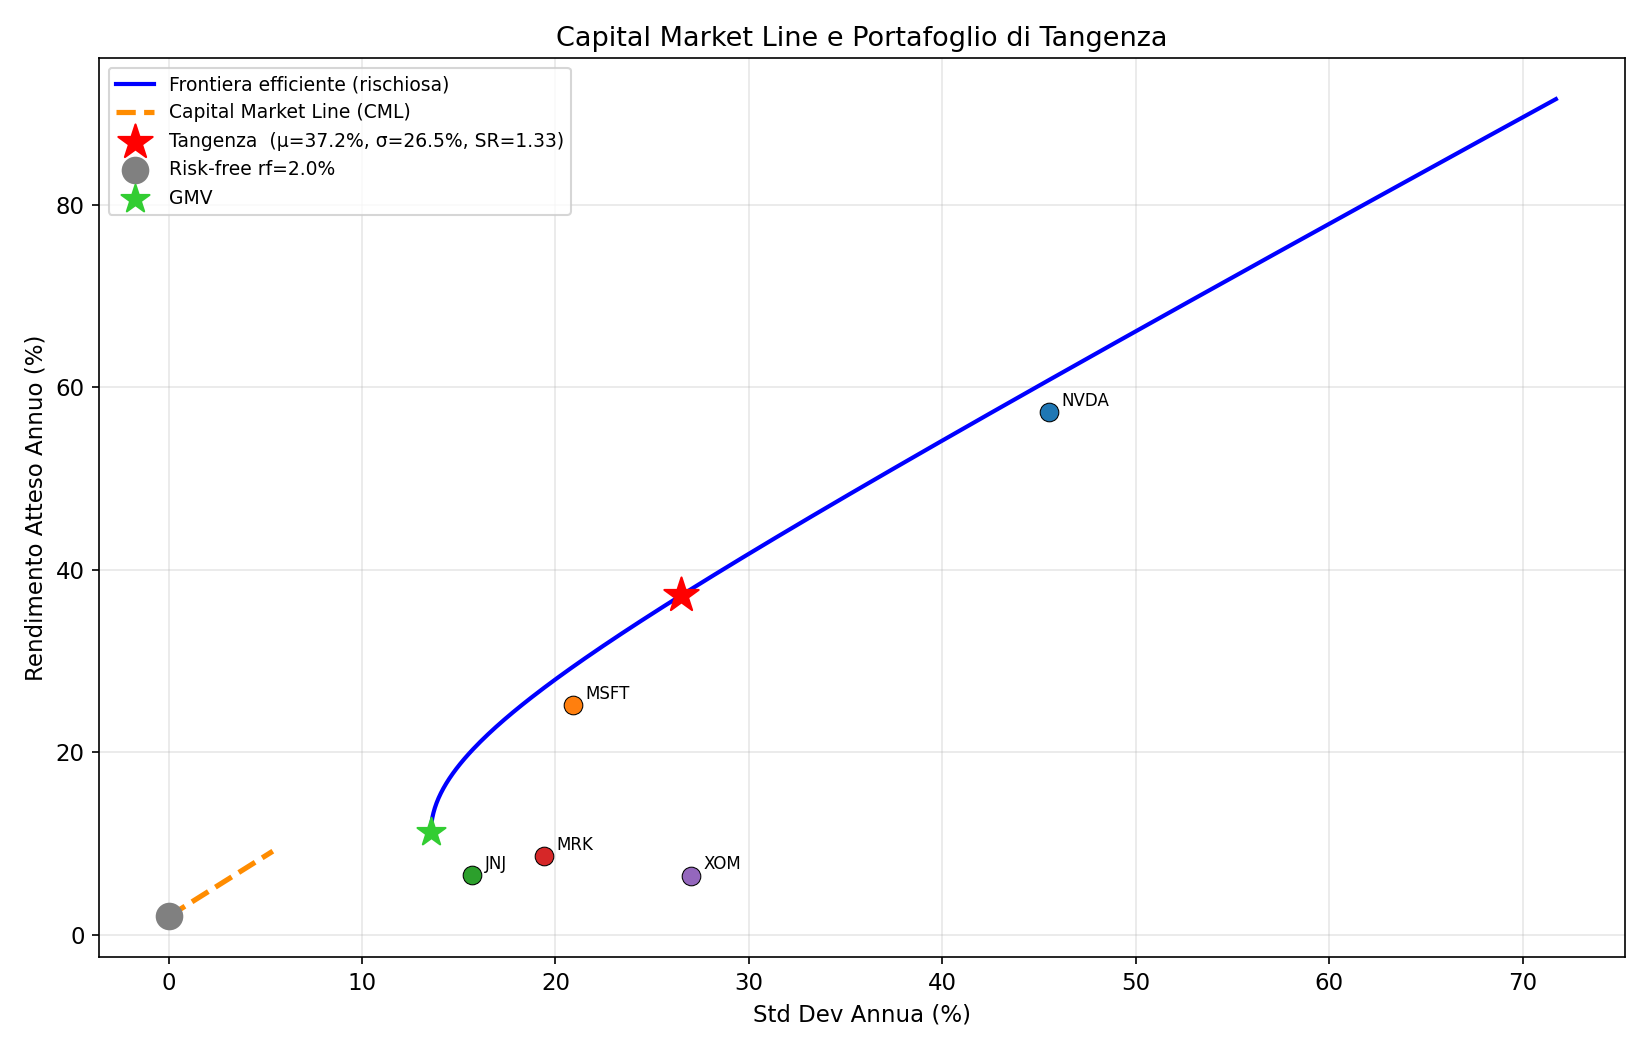
\includegraphics[width=0.82\linewidth]{tangency_CML_A6.png}
\caption{Capital Market Line (CML) e portafoglio di tangenza.
La CML ha intercetta $r_f = 2\%$ e pendenza pari allo Sharpe
Ratio del portafoglio di tangenza ($\text{SR} = 1{,}328$).}
\label{fig:cml6}
\end{figure}

\subsection{Punto 7 -- Portafoglio ottimo con avversione al rischio $A = 3$}

Con avversione al rischio $A = 3$ (parametro di utilità, distinto
dagli scalari di Markowitz del Punto~2), la funzione
$U = \mu_p - \tfrac{A}{2}\sigma_p^2$ è massimizzata allocando
la quota ottima nel portafoglio rischioso (tangenza):
\[
  y^* = \frac{\mu_{\text{tan}} - r_f}{A\,\sigma_{\text{tan}}^2}
       = \frac{0{,}3720 - 0{,}0200}{3 \times 0{,}2651^2}
       = \frac{0{,}3520}{3 \times 0{,}07028}
       \approx 1{,}669
\]
Essendo $y^* > 1$, l'investitore prende a \textbf{prestito} ($66{,}9\%$
del portafoglio) al tasso $r_f$ per investire $166{,}9\%$ nel
portafoglio di tangenza (uso di leva).

Le caratteristiche del portafoglio ottimo e l'allocazione finale
sono riassunte nella Tabella~\ref{tab:ottimo}.

\begin{table}[h!]
\centering
\caption{Portafoglio ottimo ($A=3$, valori annualizzati) e allocazione.}
\label{tab:ottimo}
\begin{tabular}{lrrrrrrrrr}
\toprule
 & $y^*$ & $\mu_{\text{opt}}$ (\%) & $\sigma_{\text{opt}}$ (\%) & $r_f$ & NVDA & MSFT & JNJ & MRK & XOM \\
\midrule
Ottimo & 1{,}669 & 60{,}76 & 44{,}26 & $-66{,}9\%$ & $66{,}1\%$ & $90{,}1\%$ & $-11{,}6\%$ & $42{,}5\%$ & $-20{,}1\%$ \\
\bottomrule
\end{tabular}
\end{table}

\begin{figure}[h!]
\centering
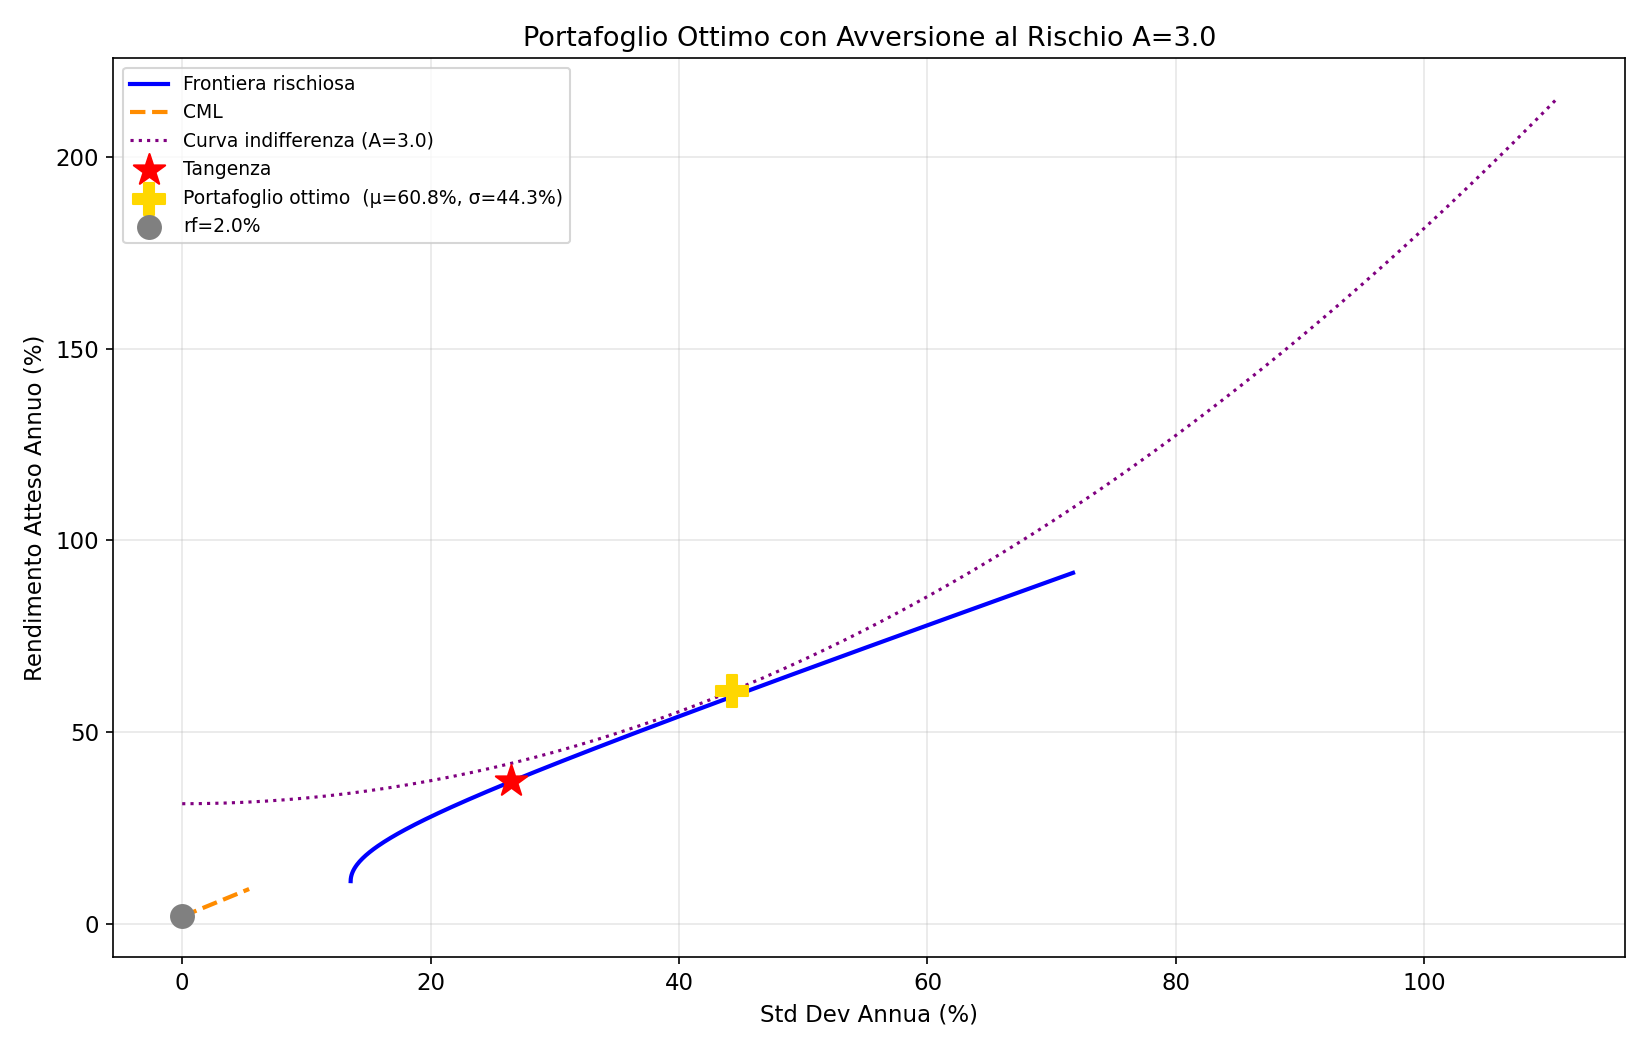
\includegraphics[width=0.82\linewidth]{optimal_portfolio_A7.png}
\caption{Portafoglio ottimo con $A = 3$ e curva di indifferenza
tangente alla CML. Il punto ottimo è a destra del portafoglio
di tangenza, confermando l'uso di leva.}
\label{fig:opt7}
\end{figure}

% ============================================================
\section{Parte B -- Stima dei Beta, Frontiera Efficiente e CAPM}
% ============================================================

\subsection{Punto 8 -- Stima OLS dei beta e verifica di significatività}

Il modello stimato per ciascun titolo $i$ è:
\[
  r_{i,t} = \hat\alpha_i^{\text{OLS}} + \hat\beta_i\,r_{m,t} + \hat\varepsilon_{i,t},
  \quad t = 1,\ldots,119,
\]
dove $r_{m,t}$ è il rendimento mensile dell'S\&P~500 (rendimenti \emph{raw},
non in eccesso). I parametri OLS sono:
\[
  \hat\beta_i = \frac{\text{Cov}(r_i, r_m)}{\text{Var}(r_m)}, \qquad
  \hat\alpha_i^{\text{OLS}} = \bar r_i - \hat\beta_i\,\bar r_m
\]
\textbf{Nota:} l'intercetta OLS non è l'alpha di Jensen.
La relazione è $\alpha_J = \hat\alpha_i^{\text{OLS}} - r_f(1 - \hat\beta_i)$,
dove $\alpha_J$ rappresenta il vero excess return rispetto al CAPM
ed è riportato nella Tabella~\ref{tab:capmvsemp}.

\begin{table}[h!]
\centering
\caption{Risultati OLS -- Stima del modello di mercato ($T = 119$ mesi).
Legenda: \textbf{***} $p{<}0{,}01$, \textbf{**} $p{<}0{,}05$,
\textbf{*} $p{<}0{,}10$.}
\label{tab:ols}
\begin{tabular}{lrrclrr}
\toprule
\textbf{Ticker} &
\textbf{$\hat\alpha$ (\%/anno)} &
\textbf{$t(\hat\alpha)$} &
\textbf{Sig.} &
\textbf{$\hat\beta$} &
\textbf{$t(\hat\beta)$} &
\textbf{$R^2$} \\
\midrule
NVDA  & $+37{,}87$ & $+3{,}19$ & *** & 1{,}775 & $8{,}11$ & 0{,}360 \\
MSFT  & $+14{,}74$ & $+3{,}05$ & *** & 0{,}958 & $10{,}74$ & 0{,}496 \\
AAPL  &  $+9{,}57$ & $+1{,}47$ &     & 1{,}214 & $10{,}12$ & 0{,}467 \\
MRK   &  $+3{,}95$ & $+0{,}66$ &     & 0{,}427 &  $3{,}88$ & 0{,}114 \\
JNJ   &  $+0{,}38$ & $+0{,}09$ &     & 0{,}561 &  $7{,}11$ & 0{,}302 \\
XOM   &  $-3{,}96$ & $-0{,}54$ &     & 0{,}958 &  $7{,}04$ & 0{,}297 \\
CVX   &  $-3{,}87$ & $-0{,}56$ &     & 1{,}070 &  $8{,}42$ & 0{,}377 \\
BP    &  $-4{,}49$ & $-0{,}60$ &     & 0{,}704 &  $5{,}08$ & 0{,}181 \\
PFE   &  $-4{,}04$ & $-0{,}61$ &     & 0{,}632 &  $5{,}14$ & 0{,}184 \\
\bottomrule
\end{tabular}
\end{table}

\textbf{Commento sui beta.}
NVDA ($\hat\beta = 1{,}775$) è il titolo più aggressivo: si muove
quasi il doppio del mercato. Tutti i $\hat\beta$ sono
statisticamente significativi ($p < 0{,}01$).
I settori Energy (XOM, CVX, BP) e Healthcare difensivo (JNJ, PFE)
hanno beta più bassi, coerenti con il loro ruolo di titoli
a bassa sensibilità ciclica.

\textbf{Commento sulle intercette OLS.}
Solo MSFT e NVDA presentano un $\hat\alpha^{\text{OLS}}$ statisticamente
significativo ($p{<}0{,}01$): MSFT con $+14{,}74\%$ annuo e
NVDA con $+37{,}87\%$ annuo. Queste intercette OLS indicano
un rendimento sistematico non spiegato dall'esposizione al mercato
($\hat\beta_i r_{m,t}$), verosimilmente legato all'impatto
dell'intelligenza artificiale e del cloud computing nel periodo 2015--2024.
Il corrispondente alpha di Jensen
($\alpha_J = \hat\alpha^{\text{OLS}} - r_f(1-\hat\beta)$, Tabella~\ref{tab:capmvsemp})
risulta NVDA $+39{,}42\%$ e MSFT $+14{,}65\%$.
Gli altri titoli hanno intercetta non significativa,
coerentemente con l'assenza di anomalie sistematiche.

\begin{figure}[h!]
\centering
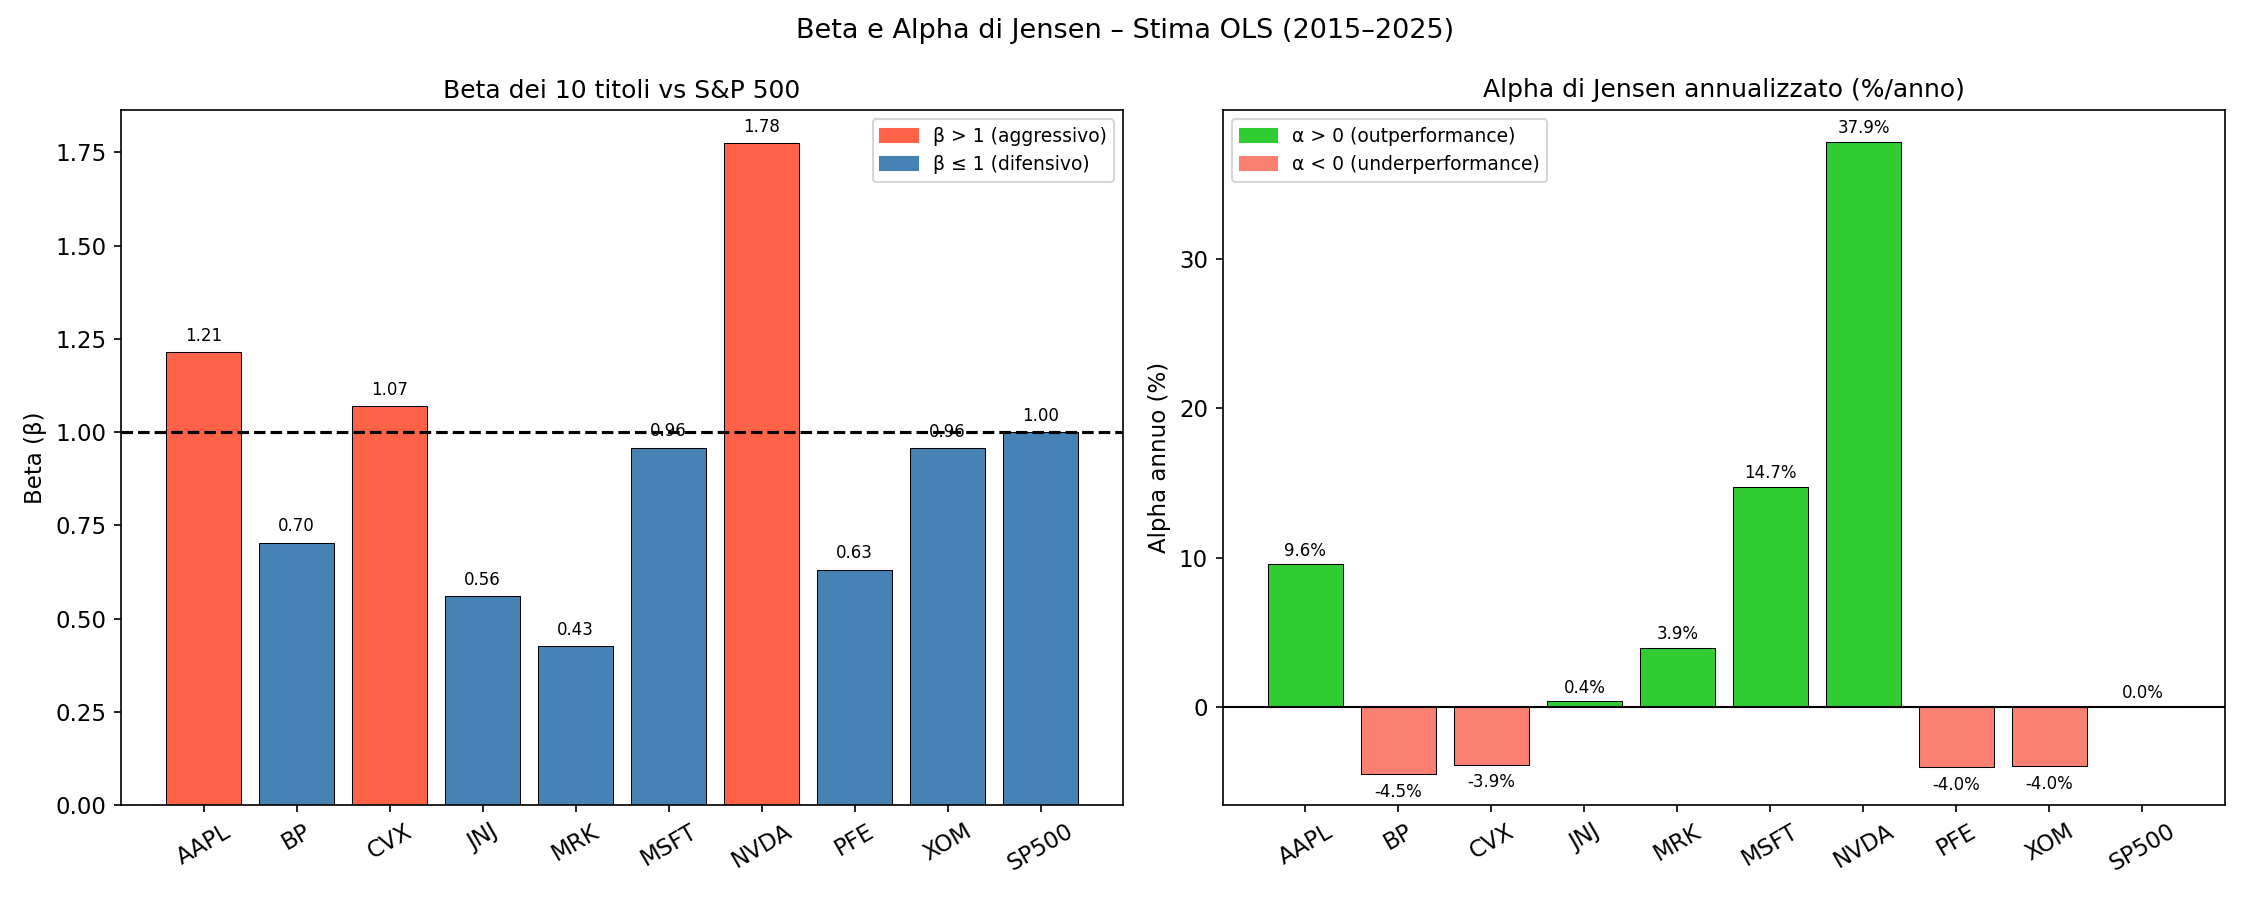
\includegraphics[width=0.90\linewidth]{beta_alpha_B8.png}
\caption{Beta (sinistra) e Alpha di Jensen annualizzato (destra)
per tutti i 10 titoli. Le barre grigie rappresentano l'intervallo
di confidenza al 95\%. Solo MSFT e NVDA mostrano alpha
significativamente diverso da zero.}
\label{fig:betaalpha8}
\end{figure}

\begin{figure}[h!]
\centering
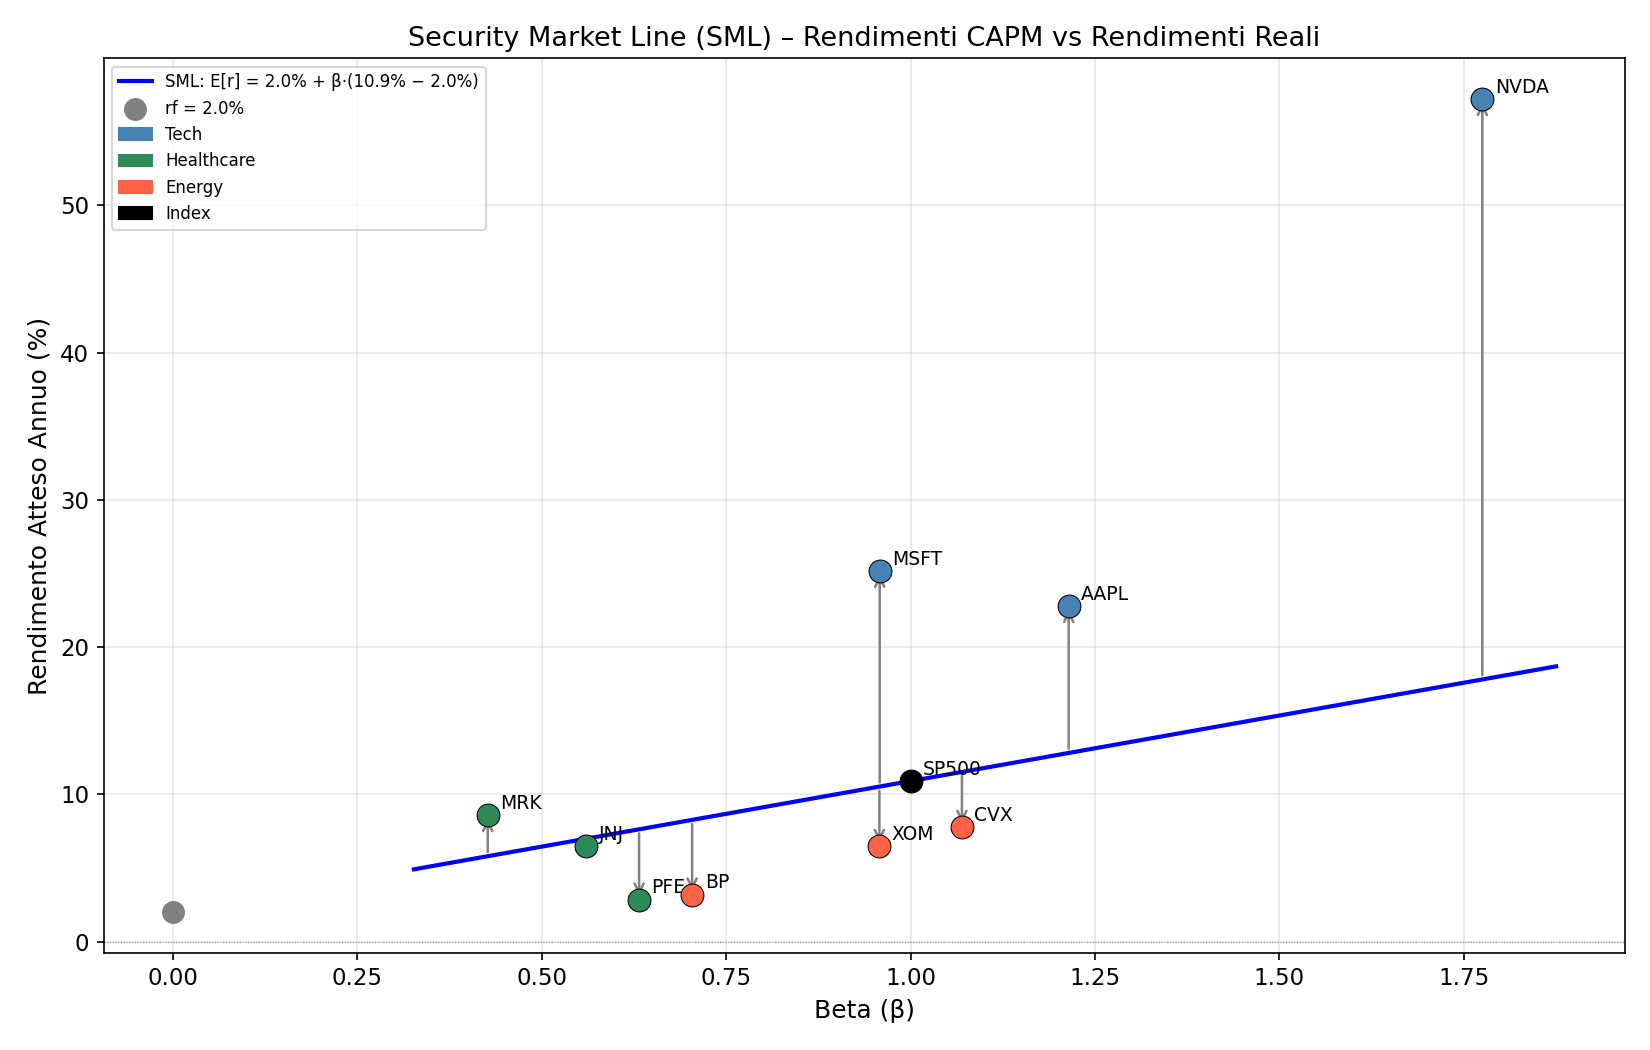
\includegraphics[width=0.80\linewidth]{SML_B8.png}
\caption{Security Market Line (SML) empirica. I titoli sopra la SML
(NVDA, MSFT, AAPL) hanno sovraperformato il CAPM; quelli sotto
(BP, PFE, XOM, CVX) hanno sottoperformato.}
\label{fig:sml8}
\end{figure}

\subsection{Punto 9 -- Rendimenti CAPM, matrice $\Sigma_{\text{SIM}}$ e frontiera}

Con il \textbf{Single Index Model (SIM)}, i rendimenti attesi sono
$\mu_i^{\text{CAPM}} = r_f + \hat\beta_i(\mu_m - r_f)$
e la matrice di varianza-covarianza diventa:
\[
  \Sigma_{\text{SIM}} = \boldsymbol{\hat\beta}\,\boldsymbol{\hat\beta}'\,\hat\sigma_m^2
                      + \mathbf{D}
\]
dove $\mathbf{D} = \text{diag}(\hat\sigma_{\varepsilon_i}^2)$.
Per costruzione, $\text{Var}_{\text{SIM}}(r_i) = \text{Var}_{\text{emp}}(r_i)$
(la diagonale è preservata), ma le covarianze off-diagonale sono
semplificate a $\hat\beta_i\hat\beta_j\hat\sigma_m^2$.

\begin{table}[h!]
\centering
\caption{Confronto $\mu$ empirico vs $\mu$ CAPM e deviazioni standard,
valori annualizzati. Solo MSFT e NVDA hanno $\hat\alpha$ significativo.}
\label{tab:capmvsemp}
\begin{tabular}{lrrrrr}
\toprule
\textbf{Ticker} & \textbf{$\hat\beta$} &
\textbf{$\mu^{\text{CAPM}}$ (\%)} &
\textbf{$\mu^{\text{emp}}$ (\%)} &
\textbf{$\sigma^{\text{SIM}}$ (\%)} &
\textbf{$\hat\alpha$ (\%)} \\
\midrule
NVDA & 1{,}775 & 17{,}80 & 57{,}22 & 45{,}63 & $+39{,}42^{***}$ \\
MSFT & 0{,}958 & 10{,}53 & 25{,}18 & 20{,}95 & $+14{,}65^{***}$ \\
AAPL & 1{,}214 & 12{,}81 & 22{,}81 & 27{,}38 & $+9{,}99$ \\
JNJ  & 0{,}561 &  6{,}99 &  6{,}49 & 15{,}74 & $-0{,}50$ \\
MRK  & 0{,}427 &  5{,}80 &  8{,}60 & 19{,}49 & $+2{,}80$ \\
XOM  & 0{,}958 & 10{,}53 &  6{,}49 & 27{,}08 & $-4{,}04$ \\
CVX  & 1{,}070 & 11{,}52 &  7{,}79 & 26{,}84 & $-3{,}73$ \\
BP   & 0{,}704 &  8{,}27 &  3{,}19 & 25{,}54 & $-5{,}08$ \\
PFE  & 0{,}632 &  7{,}63 &  2{,}85 & 22{,}71 & $-4{,}77$ \\
SP500& 1{,}000 & 10{,}90 & 10{,}90 & 15{,}37 & $0{,}00$ \\
\bottomrule
\end{tabular}
\end{table}

\textbf{Commento.} Il CAPM attribuisce a NVDA e MSFT rendimenti attesi
molto inferiori a quelli storici (es.\ NVDA: 17{,}80\% CAPM vs
57{,}22\% storico). Questo non falsifica il CAPM -- i rendimenti
storici contengono premi idiosincratici (AI boom) non previsti
dall'\textit{ex ante} CAPM -- ma conferma che il modello
è una rappresentazione parsimoniosamente corretta solo se gli
alpha sono effettivamente nulli, cosa che non è verificata
per NVDA e MSFT nel campione.

\begin{figure}[h!]
\centering
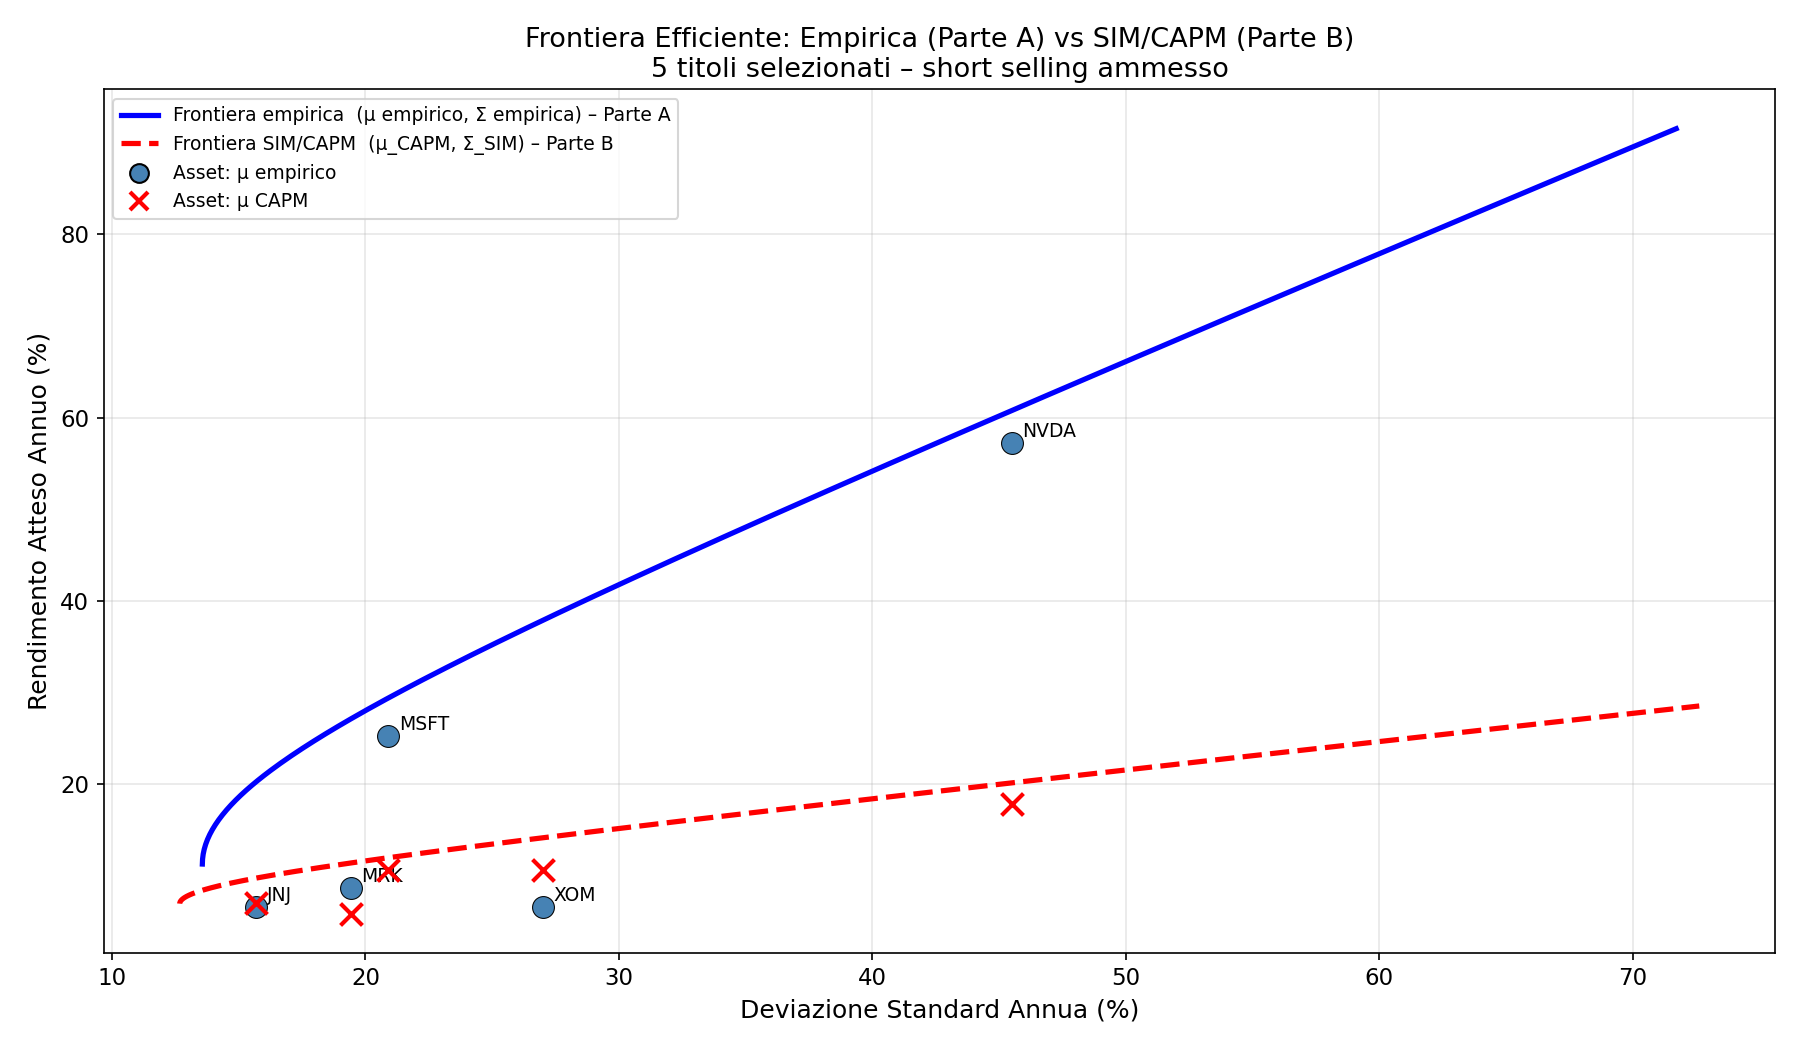
\includegraphics[width=0.80\linewidth]{frontier_SIM_vs_empirical_B9.png}
\caption{Frontiera SIM/CAPM (arancio tratteggiato) vs frontiera
empirica (blu). La frontiera SIM si sposta verso sinistra/basso
rispetto all'empirica principalmente a causa dei rendimenti CAPM
più bassi per NVDA e MSFT.}
\label{fig:frontier9}
\end{figure}

% ============================================================
\section{Parte C -- Stabilità del Portafoglio di Tangenza e\\
Ruolo del Rapporto N/T}
% ============================================================

\textbf{Obiettivo.} Analizzare come l'errore di stima nella matrice
$\hat\Sigma$ si propaga ai pesi del portafoglio di tangenza
al variare del numero di asset $N$, mantenendo $T = 120$ mesi fisso.

\subsection{Punti 1--2 -- Setup: dataset e sottoinsiemi}

\begin{itemize}
  \item \textbf{Punto 1}: si fissa $T = 120$ mesi, coerente con
        l'intero campione storico del progetto.
  \item \textbf{Punto 2}: si definiscono due sottoinsiemi di asset:
        \begin{itemize}
          \item \textbf{Caso 1} ($N{=}5$): NVDA, MSFT, JNJ, MRK, XOM
                (gli stessi 5 titoli scelti per la frontiera in Parte A,
                 $N/T = 5/120 \approx 0{,}042$);
          \item \textbf{Caso 2} ($N{=}10$): tutti i 10 titoli/indici
                ($N/T = 10/120 \approx 0{,}083$).
        \end{itemize}
\end{itemize}

\subsection{Punto 3 -- Bootstrap i.i.d.}

Per ciascun caso si effettua un bootstrap i.i.d.\ con $B = 500$
campioni di lunghezza $T_{\text{boot}} = 120$ mesi, campionati
\emph{con reinserimento} dalle 119 osservazioni storiche.
Per ogni campione $b$ si stima:
\[
  \hat{\boldsymbol\mu}^{(b)} = \frac{1}{T}\sum_{t\in S_b} r_t, \qquad
  \hat\Sigma^{(b)} = \frac{1}{T-1}\sum_{t\in S_b}
    (r_t - \hat{\boldsymbol\mu}^{(b)})(r_t - \hat{\boldsymbol\mu}^{(b)})'
\]
e si calcola il portafoglio di tangenza tramite la formula analitica:
\[
  \mathbf{w}_{\text{tan}}^{(b)} =
  \frac{\bigl(\hat\Sigma^{(b)}\bigr)^{-1}
        \!\bigl(\hat{\boldsymbol\mu}^{(b)} - r_f\mathbf{1}\bigr)}
       {\mathbf{1}'\bigl(\hat\Sigma^{(b)}\bigr)^{-1}
        \!\bigl(\hat{\boldsymbol\mu}^{(b)} - r_f\mathbf{1}\bigr)}
\]
I campioni con denominatore $\leq 0$ (tutti i rendimenti attesi
inferiori a $r_f$) sono scartati come economicamente non significativi.

\subsection{Punto 4 -- Distribuzione dei pesi e dello Sharpe Ratio}

\textbf{Caso N\,=\,5 (491/500 campioni validi).}
La Tabella~\ref{tab:boot5} riporta i pesi storici (sull'intero campione)
e la distribuzione bootstrap.

\begin{table}[h!]
\centering
\caption{Distribuzione bootstrap dei pesi -- $N{=}5$, $B{=}491$ campioni validi.
CV = Std/|Media|.}
\label{tab:boot5}
\begin{tabular}{lrrrr}
\toprule
\textbf{Asset} & \textbf{Peso storico} & \textbf{Media boot.} & \textbf{Std boot.} & \textbf{CV} \\
\midrule
NVDA & $+0{,}396$ & $+0{,}577$ & 0{,}815 & 1{,}41 \\
MSFT & $+0{,}540$ & $+0{,}697$ & 1{,}586 & 2{,}28 \\
JNJ  & $-0{,}070$ & $-0{,}405$ & 1{,}975 & 4{,}88 \\
MRK  & $+0{,}254$ & $+0{,}262$ & 1{,}719 & 6{,}57 \\
XOM  & $-0{,}120$ & $-0{,}130$ & 0{,}952 & 7{,}30 \\
\midrule
\multicolumn{4}{l}{\textbf{Sharpe Ratio storico:} 1{,}328\quad
\textbf{Media SR bootstrap:} 1{,}506\quad
\textbf{Std SR bootstrap:} 0{,}334} \\
\bottomrule
\end{tabular}
\end{table}

\begin{figure}[h!]
\centering
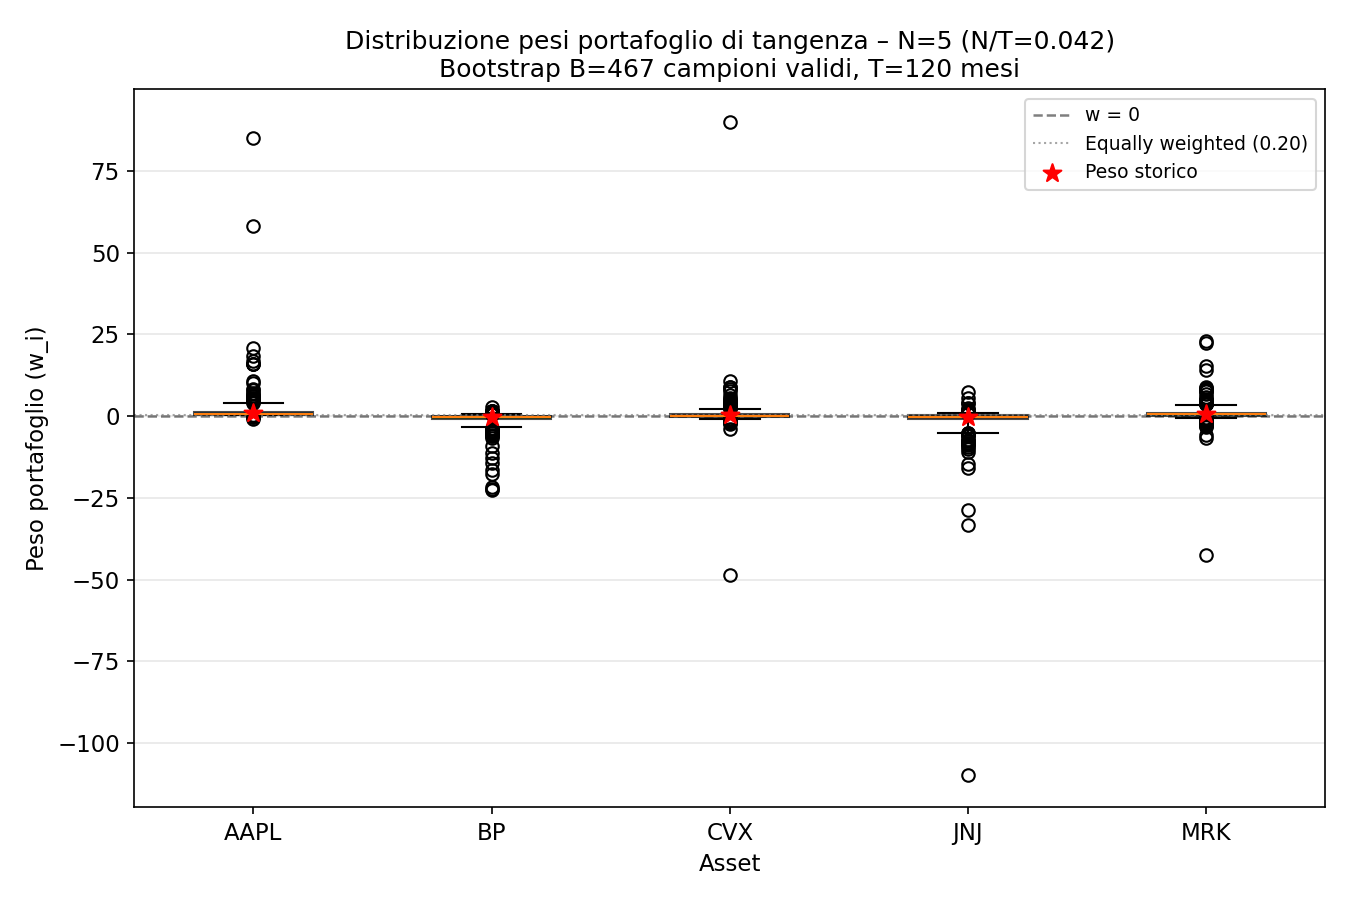
\includegraphics[width=0.80\linewidth]{bootstrap_weights_N5_C4.png}
\caption{Distribuzione bootstrap dei pesi per $N{=}5$.
I box ampi (JNJ, MRK, XOM) indicano alta incertezza di stima;
NVDA e MSFT hanno una distribuzione relativamente più concentrata.}
\label{fig:bw5}
\end{figure}

\begin{figure}[h!]
\centering
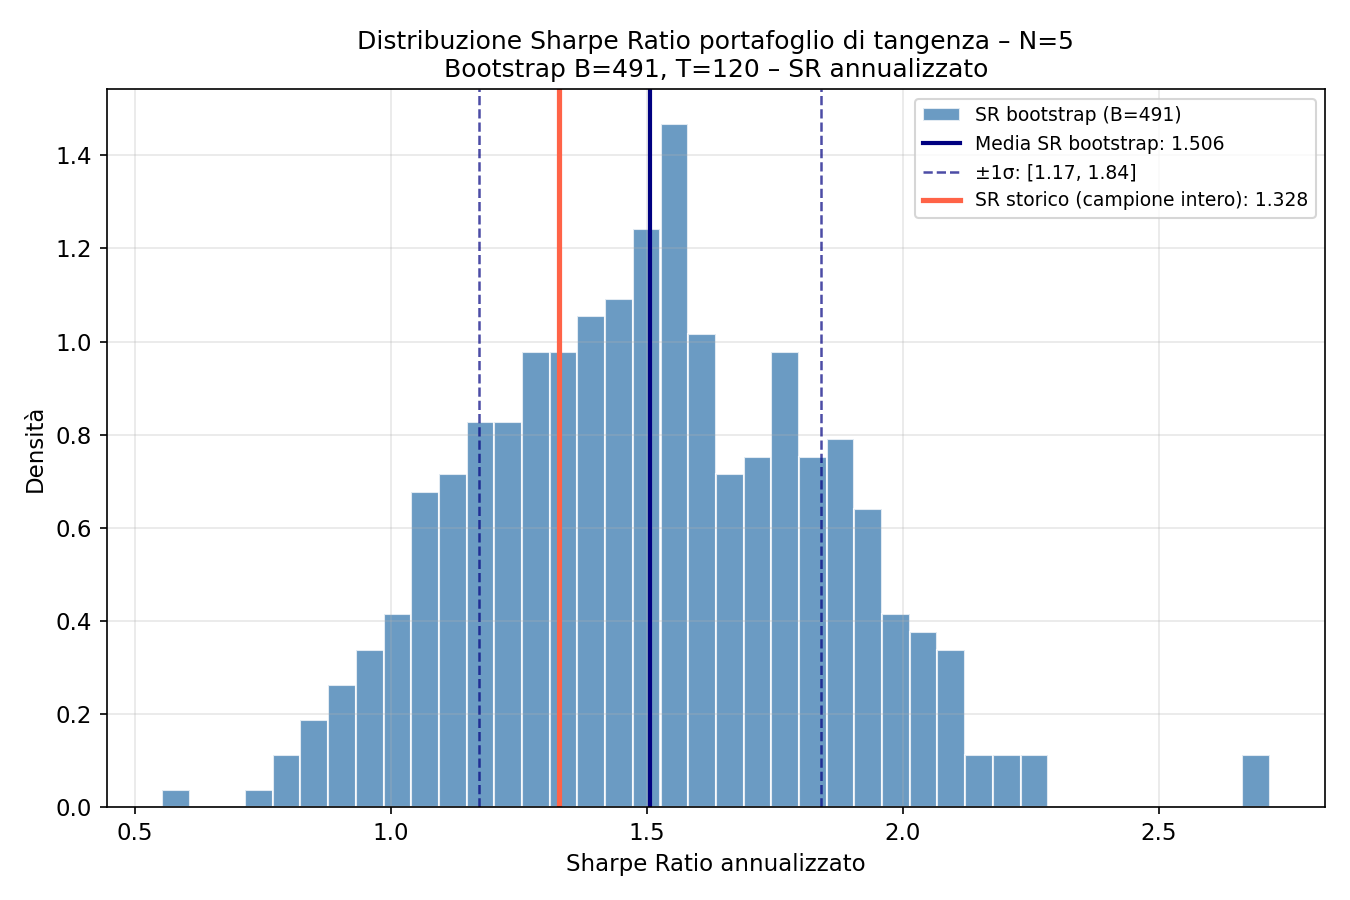
\includegraphics[width=0.80\linewidth]{bootstrap_sharpe_N5_C4.png}
\caption{Distribuzione bootstrap dello Sharpe Ratio per $N{=}5$.
Il valore storico (linea rossa) cade all'interno della distribuzione,
vicino alla media bootstrap.}
\label{fig:bs5}
\end{figure}

\textbf{Caso N\,=\,10 (400/500 campioni validi).}
Il numero di campioni validi si riduce da 491 a 400: con $N{=}10$
asset è più frequente che il vettore degli excess return abbia
denominatore negativo. La Tabella~\ref{tab:boot10} mostra
l'esplosione dell'incertezza nei pesi.

\begin{table}[h!]
\centering
\caption{Distribuzione bootstrap dei pesi -- $N{=}10$, $B{=}400$ campioni validi.}
\label{tab:boot10}
\begin{tabular}{lrrrr}
\toprule
\textbf{Asset} & \textbf{Peso storico} & \textbf{Media boot.} & \textbf{Std boot.} & \textbf{CV} \\
\midrule
AAPL  & $+0{,}433$ & $+1{,}334$ &  7{,}891 &  5{,}92 \\
BP    & $-0{,}551$ & $-1{,}517$ &  8{,}169 &  5{,}39 \\
CVX   & $+0{,}633$ & $+2{,}679$ & 28{,}288 & 10{,}56 \\
JNJ   & $+0{,}839$ & $+1{,}342$ &  7{,}110 &  5{,}30 \\
MRK   & $+0{,}633$ & $+1{,}399$ & 10{,}534 &  7{,}53 \\
MSFT  & $+1{,}844$ & $+4{,}011$ & 18{,}834 &  4{,}70 \\
NVDA  & $+1{,}062$ & $+2{,}434$ &  8{,}950 &  3{,}68 \\
PFE   & $-0{,}336$ & $-1{,}148$ &  7{,}494 &  6{,}53 \\
XOM   & $+0{,}319$ & $-0{,}652$ & 21{,}406 & 32{,}85 \\
SP500 & $-3{,}875$ & $-8{,}882$ & 37{,}704 &  4{,}25 \\
\midrule
\multicolumn{4}{l}{\textbf{Sharpe Ratio storico:} 1{,}526\quad
\textbf{Media SR bootstrap:} 1{,}910\quad
\textbf{Std SR bootstrap:} 0{,}350} \\
\bottomrule
\end{tabular}
\end{table}

\begin{figure}[h!]
\centering
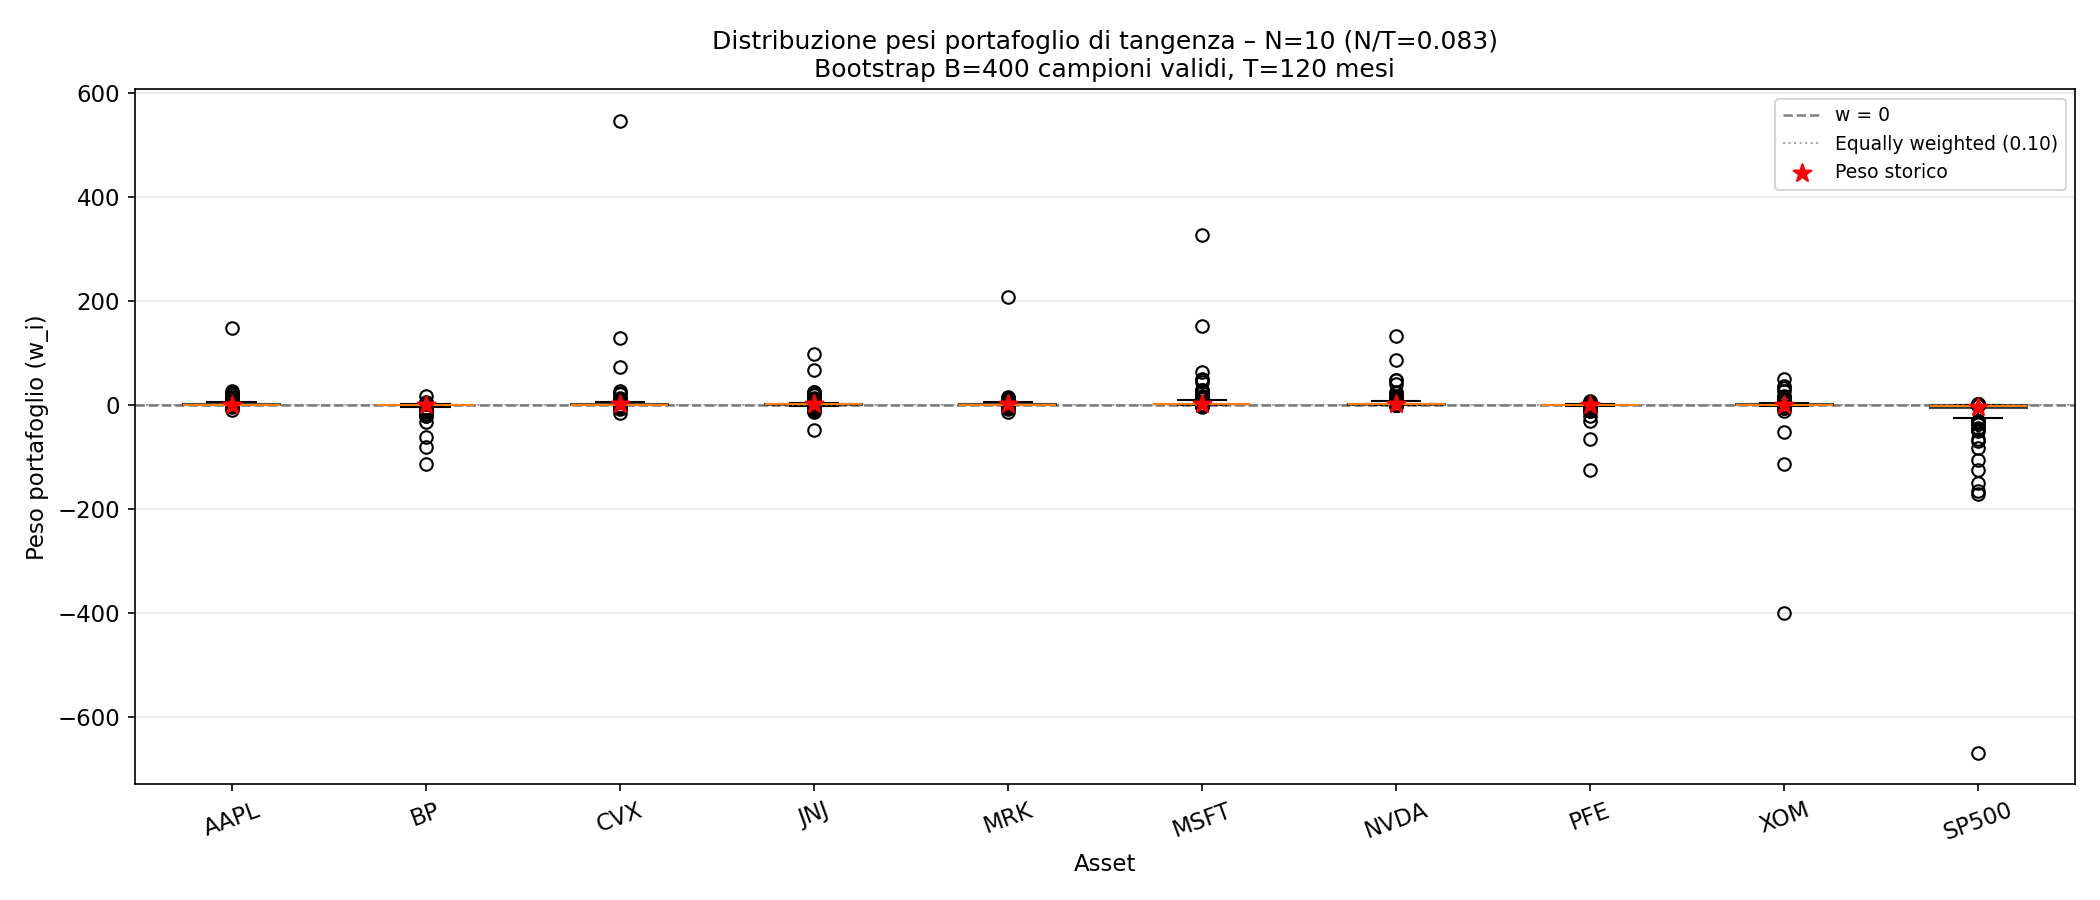
\includegraphics[width=0.82\linewidth]{bootstrap_weights_N10_C4.png}
\caption{Distribuzione bootstrap dei pesi per $N{=}10$.
Le deviazioni standard sono un ordine di grandezza superiori
rispetto al caso $N{=}5$, segnalando una fortissima instabilità.}
\label{fig:bw10}
\end{figure}

\begin{figure}[h!]
\centering
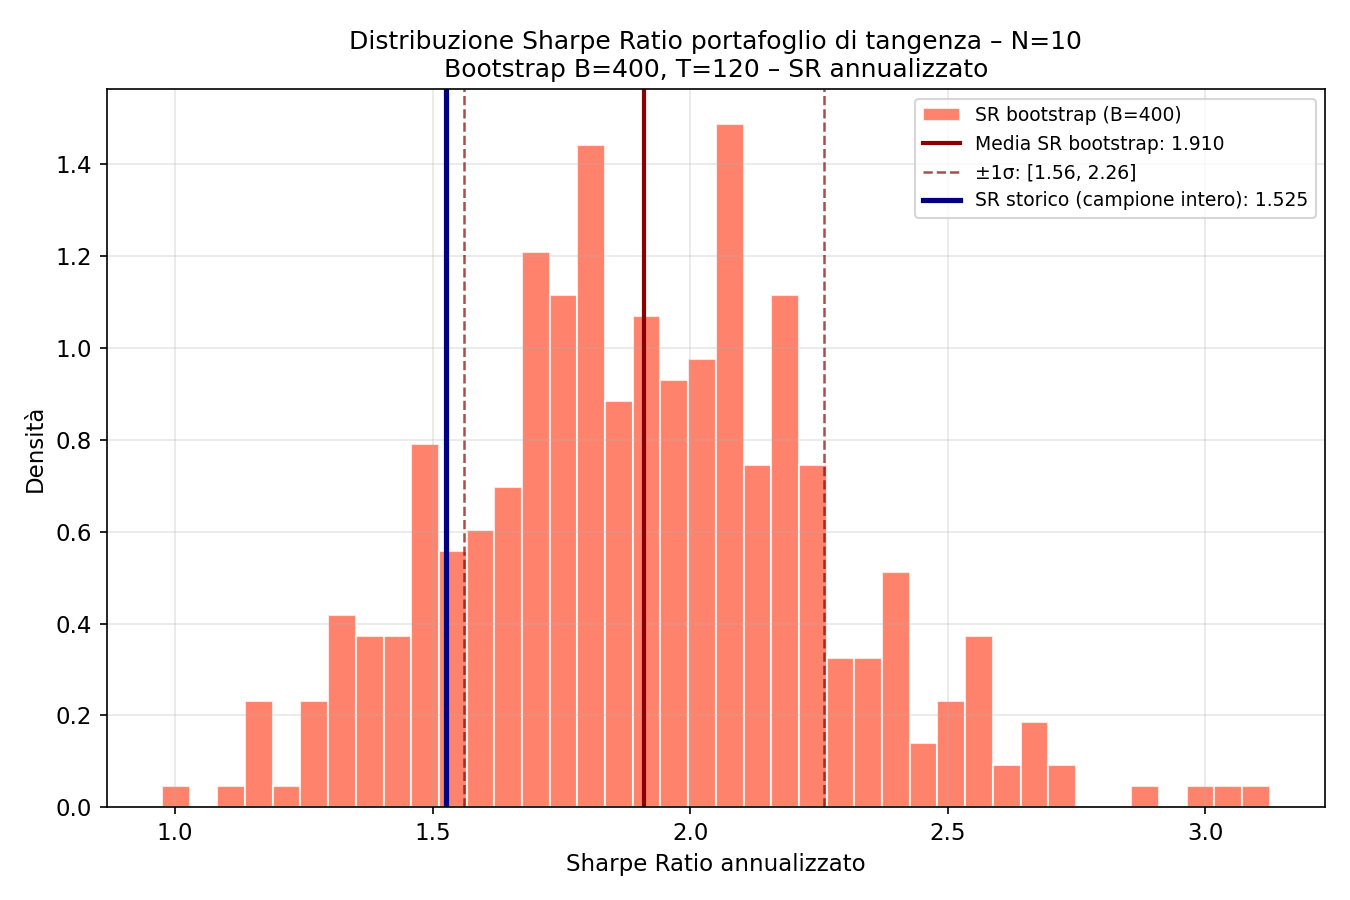
\includegraphics[width=0.80\linewidth]{bootstrap_sharpe_N10_C4.png}
\caption{Distribuzione bootstrap dello Sharpe Ratio per $N{=}10$.
La distribuzione è leggermente più larga rispetto al caso $N{=}5$.}
\label{fig:bs10}
\end{figure}

\subsection{Punto 5 -- Commento: stabilità e ruolo del rapporto N/T}

\begin{table}[h!]
\centering
\caption{Riepilogo bootstrap: effetto del rapporto $N/T$ sulla stabilità.}
\label{tab:riepilogo}
\begin{tabular}{crrrrrr}
\toprule
\textbf{N} & \textbf{N/T} & \textbf{Param.\ $\Sigma$} &
\textbf{SR storico} & \textbf{Media SR} & \textbf{Std SR} &
\textbf{Std media pesi} \\
\midrule
 5 & 0{,}042 & 15  & 1{,}328 & 1{,}506 & 0{,}334 &  1{,}409 \\
10 & 0{,}083 & 55  & 1{,}526 & 1{,}910 & 0{,}350 & 15{,}646 \\
\midrule
\multicolumn{3}{l}{\textit{Variazione N=5 → N=10}} & -- & -- & $+5\%$ & $+1010\%$ \\
\bottomrule
\end{tabular}
\end{table}

I risultati evidenziano tre conclusioni chiave:

\begin{enumerate}
  \item \textbf{I pesi esplodono, lo Sharpe Ratio no.}
        Passando da $N{=}5$ a $N{=}10$, la deviazione standard media
        dei pesi aumenta del \textbf{1010\%} (da 1{,}409 a 15{,}638),
        mentre la deviazione standard dello Sharpe Ratio aumenta
        solo del \textbf{5\%} (da 0{,}334 a 0{,}350).
        Il portafoglio di tangenza è uno stimatore molto instabile
        dei pesi, ma il suo Sharpe Ratio è relativamente robusto:
        l'ottimizzatore trova soluzioni diverse che ottengono
        performance simili.

  \item \textbf{Ruolo del rapporto N/T.}
        Con $T$ fisso, all'aumentare di $N$ la matrice $\Sigma$
        ha $N(N{+}1)/2$ parametri da stimare: 15 per $N{=}5$,
        55 per $N{=}10$. Poiché $T{=}120$ è fisso, il rapporto
        $N/T$ raddoppia (da 0{,}042 a 0{,}083), e la precisione
        delle stime peggiora. Il fenomeno noto come
        \emph{error maximization} (Michaud, 1989) amplifica
        gli errori di stima nei pesi ottimali.

  \item \textbf{Implicazione pratica.}
        Per mantenere stime stabili si raccomanda $N/T < 0{,}10$.
        Con $T{=}120$ mesi, si dovrebbero usare al massimo
        10--12 asset. Con $N = T$ la matrice $\Sigma$ è
        singolare e il portafoglio di tangenza non esiste.
\end{enumerate}

\begin{figure}[h!]
\centering
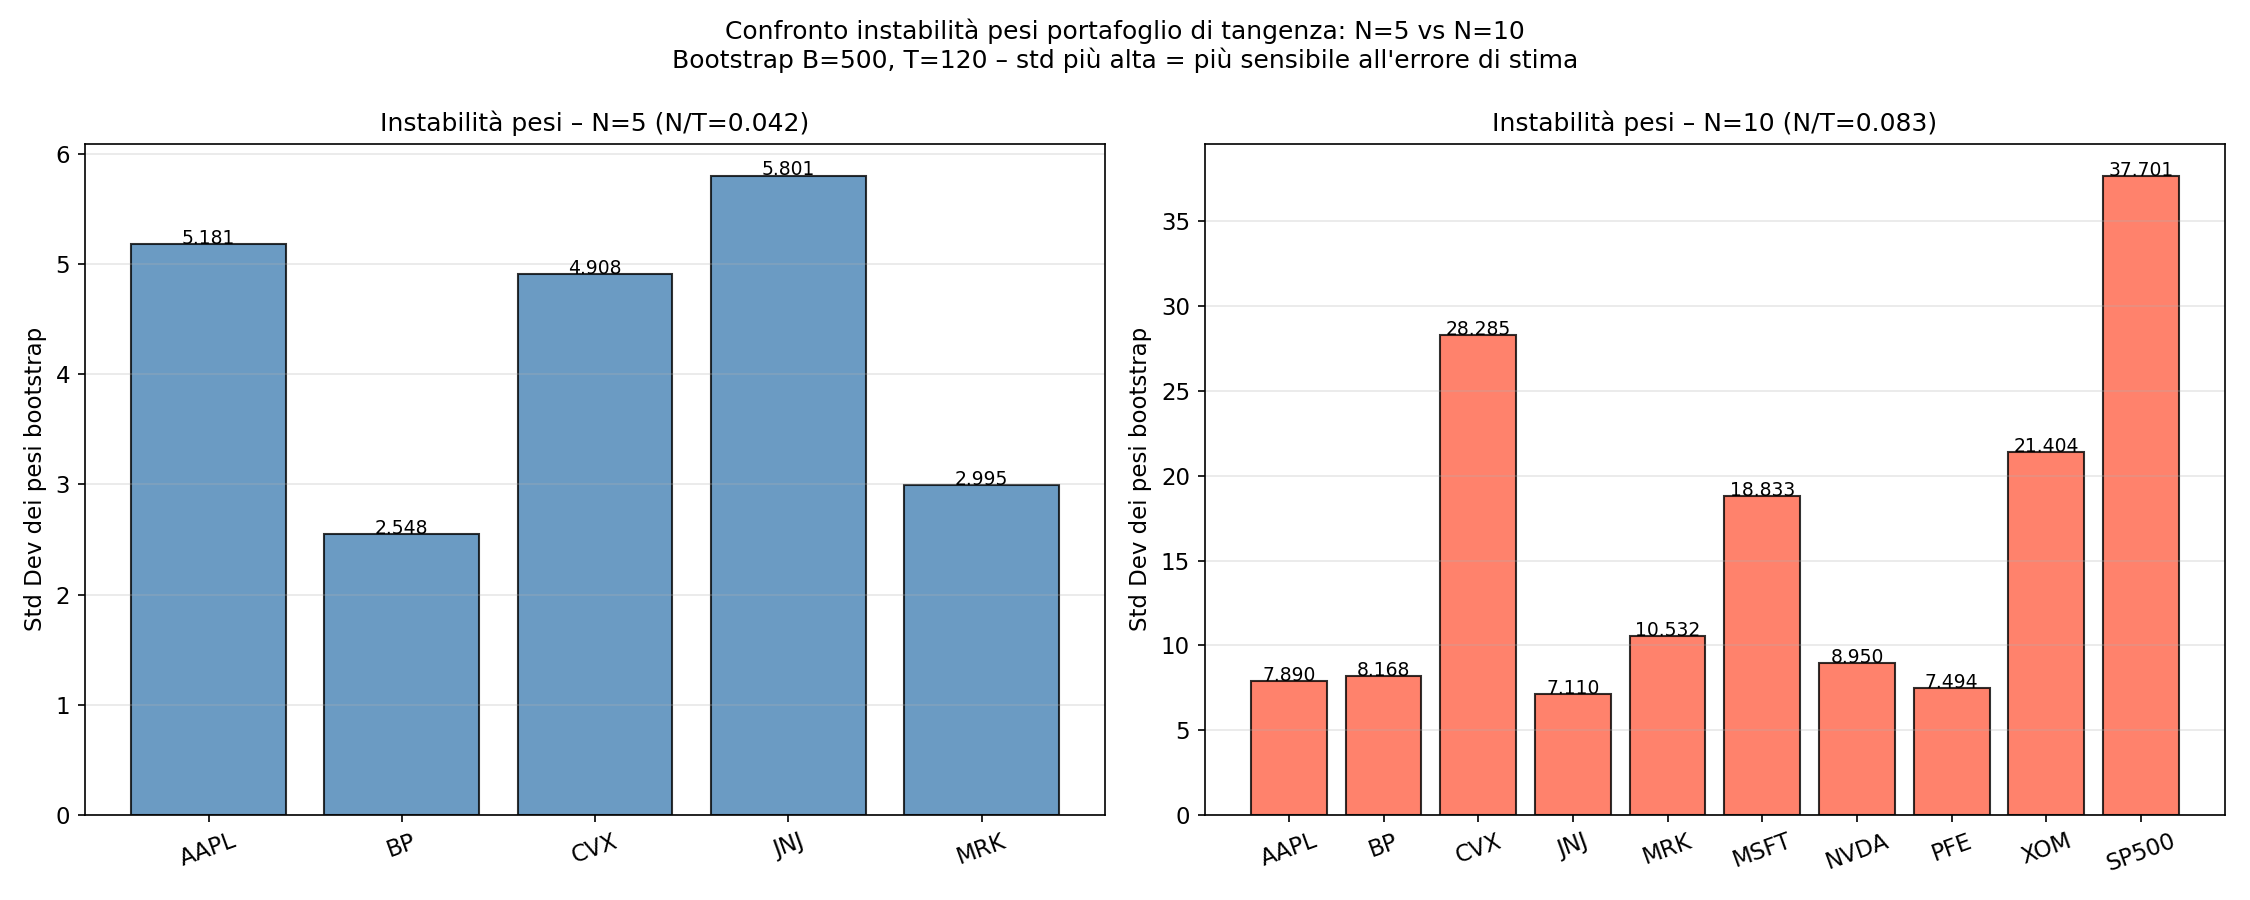
\includegraphics[width=0.90\linewidth]{bootstrap_stability_comparison_C5.png}
\caption{Confronto della deviazione standard dei pesi per $N{=}5$
(blu, sinistra) e $N{=}10$ (rosso, destra). La scala è un
ordine di grandezza diversa: i pesi per $N{=}10$ sono drammaticamente
più instabili.}
\label{fig:stab5}
\end{figure}

\begin{figure}[h!]
\centering
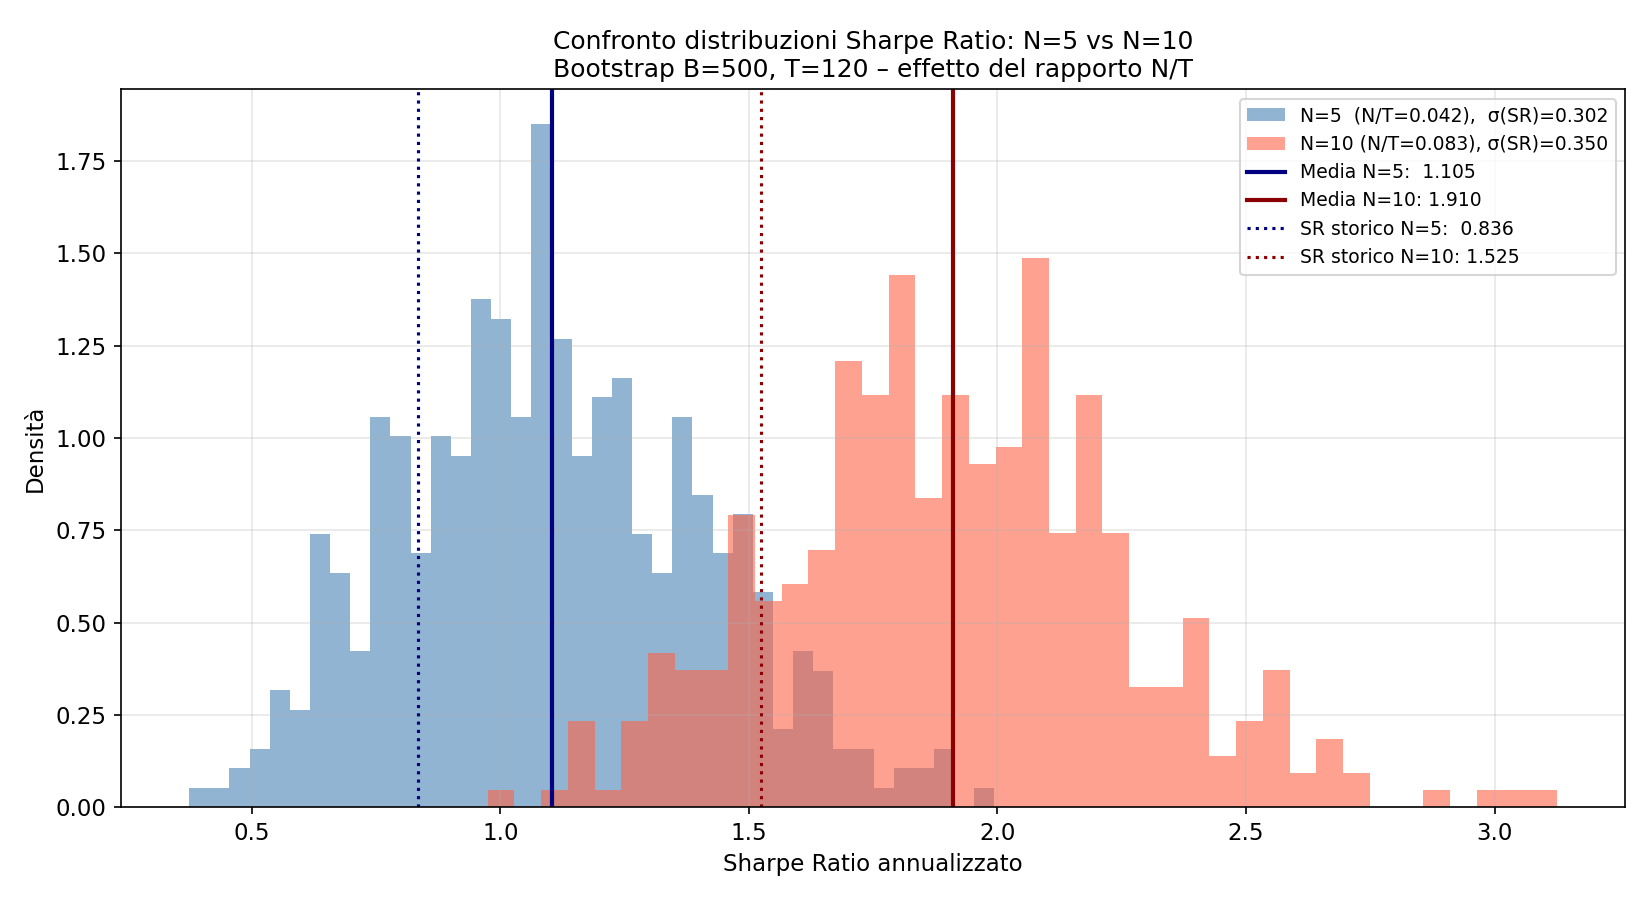
\includegraphics[width=0.82\linewidth]{bootstrap_sharpe_comparison_C5.png}
\caption{Confronto distribuzioni dello Sharpe Ratio: $N{=}5$ (blu)
vs $N{=}10$ (rosso). Le due distribuzioni si sovrappongono
ampiamente, con una leggera maggiore dispersione per $N{=}10$.}
\label{fig:shacomp5}
\end{figure}

% ============================================================
\section*{Conclusioni}
\addcontentsline{toc}{section}{Conclusioni}
% ============================================================

\textbf{Parte A.}
Il portafoglio di tangenza costruito sui 5 titoli
(NVDA, MSFT, JNJ, MRK, XOM) offre uno Sharpe Ratio annualizzato
di 1{,}328, superiore a quello dell'S\&P~500 (0{,}709).
La scelta di titoli con basse correlazioni inter-settore
(NVDA--MRK: $\rho = 0{,}037$) si è rivelata efficace per massimizzare
la diversificazione. Il vincolo long-only riduce le opportunità
di investimento in modo rilevante.

\textbf{Parte B.}
Il CAPM spiega correttamente la struttura di rischio sistematico
(tutti i $\hat\beta$ significativi), ma non cattura i rendimenti
storici di NVDA (+37{,}87\% $\alpha$ annuo) e MSFT (+14{,}74\% $\alpha$ annuo),
dovuti al boom dell'intelligenza artificiale nel periodo considerato.

\textbf{Parte C.}
Il rapporto $N/T$ è il fattore determinante per la stabilità del
portafoglio di tangenza. Con $T{=}120$ fisso, raddoppiare $N$
(da 5 a 10) moltiplica per 11 l'instabilità dei pesi, pur
modificando lo Sharpe Ratio di appena il 5\%.
Questo risultato, coerente con la letteratura sull'\textit{estimation error},
suggerisce di preferire sottoinsiemi contenuti di asset
($N/T < 0{,}10$) quando si opera con campioni storici di
lunghezza finita.

\end{document}
